%\SweaveUTF8
\documentclass[aspectratio=169]{beamer}
\usepackage{Sweave}

\usetheme{default}
% Slide setup, colour independent

\usepackage{amsmath,amssymb,amsthm}
\usepackage[utf8]{inputenc}
\usepackage{colortbl}
\usepackage{bm}
\usepackage{xcolor}
\usepackage{dsfont}
\usepackage{setspace}
%\usepackage{subfigure}
% To use \ding{234} and the like
\usepackage{pifont}
% To cross reference between slide files
\usepackage{zref-xr,zref-user}
% Use something like
% \zexternaldocument{fileI}
% in the tex files. And cite using \zref instead of \ref

% Fields and the like
\def\IC{\mathbb{C}}
\def\IF{\mathbb{F}}
\def\II{\mathbb{I}}
\def\IJ{\mathbb{J}}
\def\IM{\mathbb{M}}
\def\IN{\mathbb{N}}
\def\IP{\mathbb{P}}
\def\IR{\mathbb{R}}
\def\IZ{\mathbb{Z}}
\def\11{\mathds{1}}


% Bold lowercase
\def\ba{\bm{a}}
\def\bb{\bm{b}}
\def\bc{\bm{c}}
\def\bd{\bm{d}}
\def\be{\bm{e}}
\def\bf{\bm{f}}
\def\bh{\bm{h}}
\def\bi{\bm{i}}
\def\bj{\bm{j}}
\def\bk{\bm{k}}
\def\bn{\bm{n}}
\def\bp{\bm{p}}
\def\br{\bm{r}}
\def\bs{\bm{s}}
\def\bu{\bm{u}}
\def\bv{\bm{v}}
\def\bw{\bm{w}}
\def\bx{\bm{x}}
\def\by{\bm{y}}
\def\bz{\bm{z}}

% Bold capitals
\def\bB{\bm{B}}
\def\bD{\bm{D}}
\def\bE{\bm{E}}
\def\bF{\bm{F}}
\def\bG{\bm{G}}
\def\bI{\bm{I}}
\def\bL{\bm{L}}
\def\bN{\bm{N}}
\def\bP{\bm{P}}
\def\bR{\bm{R}}
\def\bS{\bm{S}}
\def\bT{\bm{T}}
\def\bX{\bm{X}}

% Bold numbers
\def\b0{\bm{0}}

% Bold greek
\bmdefine{\bmu}{\bm{\mu}}
\def\bphi{\bm{\phi}}
\def\bvarphi{\bm{\varphi}}
\def\bPi{\bm{\Pi}}
\def\bGamma{\bm{\Gamma}}

% Bold red sentence
\def\boldred#1{{\color{red}\textbf{#1}}}
\def\defword#1{{\color{orange}\textbf{#1}}}

% Caligraphic letters
\def\A{\mathcal{A}}
\def\B{\mathcal{B}}
\def\C{\mathcal{C}}
\def\D{\mathcal{D}}
\def\E{\mathcal{E}}
\def\F{\mathcal{F}}
\def\G{\mathcal{G}}
\def\H{\mathcal{H}}
\def\I{\mathcal{I}}
\def\L{\mathcal{L}}
\def\M{\mathcal{M}}
\def\N{\mathcal{N}}
\def\P{\mathcal{P}}
\def\R{\mathcal{R}}
\def\S{\mathcal{S}}
\def\T{\mathcal{T}}
\def\U{\mathcal{U}}
\def\V{\mathcal{V}}

% Adding space for prime (') where needed
\def\pprime{\,'}
% Adding space for star (\star) where needed
\def\pstar{{\,\star}}

% tt font for code
\def\code#1{{\tt #1}}

% i.e., e.g.
\def\eg{\emph{e.g.}}
\def\ie{\emph{i.e.}}


% Operators and special symbols
\def\nbOne{{\mathchoice {\rm 1\mskip-4mu l} {\rm 1\mskip-4mu l}
{\rm 1\mskip-4.5mu l} {\rm 1\mskip-5mu l}}}
\def\cov{\ensuremath{\mathsf{cov}}}
\def\Var{\ensuremath{\mathsf{Var}\ }}
\def\Im{\textrm{Im}\;}
\def\Re{\textrm{Re}\;}
\def\det{\ensuremath{\mathsf{det}}}
\def\diag{\ensuremath{\mathsf{diag}}}
\def\nullspace{\ensuremath{\mathsf{null}}}
\def\nullity{\ensuremath{\mathsf{nullity}}}
\def\rank{\ensuremath{\mathsf{rank}}}
\def\range{\ensuremath{\mathsf{range}}}
\def\sgn{\ensuremath{\mathsf{sgn}}}
\def\Span{\ensuremath{\mathsf{span}}}
\def\tr{\ensuremath{\mathsf{tr}}}
\def\imply{$\Rightarrow$}
\def\restrictTo#1#2{\left.#1\right|_{#2}}
\newcommand{\parallelsum}{\mathbin{\!/\mkern-5mu/\!}}
\def\dsum{\mathop{\displaystyle \sum }}%
\def\dind#1#2{_{\substack{#1\\ #2}}}

\DeclareMathOperator{\GL}{GL}
\DeclareMathOperator{\Rel}{Re}
\def\Nt#1{\left|\!\left|\!\left|#1\right|\!\right|\!\right|}
\newcommand{\tripbar}{|\! |\! |}



% The beamer bullet (in base colour)
\def\bbullet{\leavevmode\usebeamertemplate{itemize item}\ }

% Theorems and the like
\newtheorem{proposition}[theorem]{Proposition}
\newtheorem{property}[theorem]{Property}
\newtheorem{importantproperty}[theorem]{Property}
\newtheorem{importanttheorem}[theorem]{Theorem}
%\newtheorem{lemma}[theorem]{Lemma}
%\newtheorem{corollary}[theorem]{Corollary}
\newtheorem{remark}[theorem]{Remark}
\setbeamertemplate{theorems}[numbered]
%\setbeamertemplate{theorems}[ams style]

%
%\usecolortheme{orchid}
%\usecolortheme{orchid}

\def\red{\color[rgb]{1,0,0}}
\def\blue{\color[rgb]{0,0,1}}
\def\green{\color[rgb]{0,1,0}}


% Get rid of navigation stuff
\setbeamertemplate{navigation symbols}{}

% Set footline/header line
\setbeamertemplate{footline}
{%
\quad p. \insertpagenumber \quad--\quad \insertsection\vskip2pt
}
% \setbeamertemplate{headline}
% {%
% \quad\insertsection\hfill p. \insertpagenumber\quad\mbox{}\vskip2pt
% }


\makeatletter
\newlength\beamerleftmargin
\setlength\beamerleftmargin{\Gm@lmargin}
\makeatother

% Colours for special pages
\def\extraContent{yellow!20}


%%%%%%%%%%%%%%%%%
\usepackage{tikz}
\usetikzlibrary{shapes,arrows}
\usetikzlibrary{positioning}
\usetikzlibrary{shapes.symbols,shapes.callouts,patterns}
\usetikzlibrary{calc,fit}
\usetikzlibrary{backgrounds}
\usetikzlibrary{decorations.pathmorphing,fit,petri}
\usetikzlibrary{automata}
\usetikzlibrary{fadings}
\usetikzlibrary{patterns,hobby}
\usetikzlibrary{backgrounds,fit,petri}


\usepackage{pgfplots}
\pgfplotsset{compat=1.6}
\pgfplotsset{ticks=none}

\usetikzlibrary{decorations.markings}
\usetikzlibrary{arrows.meta}
\tikzset{>=stealth}

% For tikz
\tikzstyle{cloud} = [draw, ellipse,fill=red!20, node distance=0.87cm,
minimum height=2em]
\tikzstyle{line} = [draw, -latex']


%%% For max frame images
\newenvironment{changemargin}[2]{%
\begin{list}{}{%
\setlength{\topsep}{0pt}%
\setlength{\leftmargin}{#1}%
\setlength{\rightmargin}{#2}%
\setlength{\listparindent}{\parindent}%
\setlength{\itemindent}{\parindent}%
\setlength{\parsep}{\parskip}%
}%
\item[]}{\end{list}}


% Make one image take up the entire slide content area in beamer,.:
% centered/centred full-screen image, with title:
% This uses the whole screen except for the 1cm border around it
% all. 128x96mm
\newcommand{\titledFrameImage}[2]{
\begin{frame}{#1}
%\begin{changemargin}{-1cm}{-1cm}
\begin{center}
\includegraphics[width=108mm,height=\textheight,keepaspectratio]{#2}
\end{center}
%\end{changemargin}
\end{frame}
}

% Make one image take up the entire slide content area in beamer.:
% centered/centred full-screen image, no title:
% This uses the whole screen except for the 1cm border around it
% all. 128x96mm
\newcommand{\plainFrameImage}[1]{
\begin{frame}[plain]
%\begin{changemargin}{-1cm}{-1cm}
\begin{center}
\includegraphics[width=108mm,height=76mm,keepaspectratio]{#1}
\end{center}
%\end{changemargin}
\end{frame}
}

% Make one image take up the entire slide area, including borders, in beamer.:
% centered/centred full-screen image, no title:
% This uses the entire whole screen
\newcommand{\maxFrameImage}[1]{
\begin{frame}[plain]
\begin{changemargin}{-1cm}{-1cm}
\begin{center}
\includegraphics[width=\paperwidth,height=\paperheight,keepaspectratio]
{#1}
\end{center}
\end{changemargin}
\end{frame}
}

% This uses the entire whole screen (to include in frame)
\newcommand{\maxFrameImageNoFrame}[1]{
\begin{changemargin}{-1cm}{-1cm}
\begin{center}
\includegraphics[width=\paperwidth,height=0.99\paperheight,keepaspectratio]
{#1}
\end{center}
\end{changemargin}
}

% Make one image take up the entire slide area, including borders, in beamer.:
% centered/centred full-screen image, no title:
% This uses the entire whole screen
\newcommand{\maxFrameImageColor}[2]{
\begin{frame}[plain]
\setbeamercolor{normal text}{bg=#2!20}
\begin{changemargin}{-1cm}{-1cm}
\begin{center}
\includegraphics[width=\paperwidth,height=\paperheight,keepaspectratio]
{#1}
\end{center}
\end{changemargin}
\end{frame}
}


\usepackage{tikz}
\usetikzlibrary{patterns,hobby}
\usepackage{pgfplots}
\pgfplotsset{compat=1.6}
\pgfplotsset{ticks=none}

\usetikzlibrary{backgrounds}
\usetikzlibrary{decorations.markings}
\usetikzlibrary{arrows.meta}
\tikzset{>=stealth}

\tikzset{
  clockwise arrows/.style={
    postaction={
      decorate,
      decoration={
        markings,
        mark=between positions 0.1 and 0.9 step 40pt with {\arrow{>}},
   }}}}


   %%%%%%%%%%%
% To have links to parts in the outline
\makeatletter
\AtBeginPart{%
  \addtocontents{toc}{\protect\beamer@partintoc{\the\c@part}{\beamer@partnameshort}{\the\c@page}}%
}
%% number, shortname, page.
\providecommand\beamer@partintoc[3]{%
  \ifnum\c@tocdepth=-1\relax
    % requesting onlyparts.
    \makebox[6em]{Part #1:} \textcolor{green!30!blue}{\hyperlink{#2}{#2}}
    \par
  \fi
}
\define@key{beamertoc}{onlyparts}[]{%
  \c@tocdepth=-1\relax
}
\makeatother%

\newcommand{\nameofthepart}{}
\newcommand{\nupart}[1]%
    {   \part{#1}%
        \renewcommand{\nameofthepart}{#1}%
        {
          \setbeamercolor{background canvas}{bg=orange!50}
          \begin{frame}{#1}%\partpage 
          \hypertarget{\nameofthepart}{}\tableofcontents%
          \end{frame}
        }
    }



\usecolortheme{orchid}
%% Listings
\usepackage{listings}
\definecolor{mygreen}{rgb}{0,0.6,0}
\definecolor{mygray}{rgb}{0.5,0.5,0.5}
\definecolor{mymauve}{rgb}{0.58,0,0.82}
\definecolor{mygold}{rgb}{1,0.843,0}
\definecolor{myblue}{rgb}{0.537,0.812,0.941}

\definecolor{lgreen}{rgb}{0.6,0.9,.6}
\definecolor{lred}{rgb}{1,0.5,.5}

\lstloadlanguages{R}
\lstset{ %
  language=R,
  backgroundcolor=\color{black!05},   % choose the background color
  basicstyle=\footnotesize\ttfamily,        % size of fonts used for the code
  breaklines=true,                 % automatic line breaking only at whitespace
  captionpos=b,                    % sets the caption-position to bottom
  commentstyle=\color{mygreen},    % comment style
  escapeinside={\%*}{*)},          % if you want to add LaTeX within your code
  keywordstyle=\color{red},       % keyword style
  stringstyle=\color{mygold},     % string literal style
  keepspaces=true,
  columns=fullflexible,
  tabsize=4,
}
% Could also do (in lstset)
% basicstyle==\fontfamily{pcr}\footnotesize
\lstdefinelanguage{Renhanced}%
  {keywords={abbreviate,abline,abs,acos,acosh,action,add1,add,%
      aggregate,alias,Alias,alist,all,anova,any,aov,aperm,append,apply,%
      approx,approxfun,apropos,Arg,args,array,arrows,as,asin,asinh,%
      atan,atan2,atanh,attach,attr,attributes,autoload,autoloader,ave,%
      axis,backsolve,barplot,basename,besselI,besselJ,besselK,besselY,%
      beta,binomial,body,box,boxplot,break,browser,bug,builtins,bxp,by,%
      c,C,call,Call,case,cat,category,cbind,ceiling,character,char,%
      charmatch,check,chol,chol2inv,choose,chull,class,close,cm,codes,%
      coef,coefficients,co,col,colnames,colors,colours,commandArgs,%
      comment,complete,complex,conflicts,Conj,contents,contour,%
      contrasts,contr,control,helmert,contrib,convolve,cooks,coords,%
      distance,coplot,cor,cos,cosh,count,fields,cov,covratio,wt,CRAN,%
      create,crossprod,cummax,cummin,cumprod,cumsum,curve,cut,cycle,D,%
      data,dataentry,date,dbeta,dbinom,dcauchy,dchisq,de,debug,%
      debugger,Defunct,default,delay,delete,deltat,demo,de,density,%
      deparse,dependencies,Deprecated,deriv,description,detach,%
      dev2bitmap,dev,cur,deviance,off,prev,,dexp,df,dfbetas,dffits,%
      dgamma,dgeom,dget,dhyper,diag,diff,digamma,dim,dimnames,dir,%
      dirname,dlnorm,dlogis,dnbinom,dnchisq,dnorm,do,dotplot,double,%
      download,dpois,dput,drop,drop1,dsignrank,dt,dummy,dump,dunif,%
      duplicated,dweibull,dwilcox,dyn,edit,eff,effects,eigen,else,%
      emacs,end,environment,env,erase,eval,equal,evalq,example,exists,%
      exit,exp,expand,expression,External,extract,extractAIC,factor,%
      fail,family,fft,file,filled,find,fitted,fivenum,fix,floor,for,%
      For,formals,format,formatC,formula,Fortran,forwardsolve,frame,%
      frequency,ftable,ftable2table,function,gamma,Gamma,gammaCody,%
      gaussian,gc,gcinfo,gctorture,get,getenv,geterrmessage,getOption,%
      getwd,gl,glm,globalenv,gnome,GNOME,graphics,gray,grep,grey,grid,%
      gsub,hasTsp,hat,heat,help,hist,home,hsv,httpclient,I,identify,if,%
      ifelse,Im,image,\%in\%,index,influence,measures,inherits,install,%
      installed,integer,interaction,interactive,Internal,intersect,%
      inverse,invisible,IQR,is,jitter,kappa,kronecker,labels,lapply,%
      layout,lbeta,lchoose,lcm,legend,length,levels,lgamma,library,%
      licence,license,lines,list,lm,load,local,locator,log,log10,log1p,%
      log2,logical,loglin,lower,lowess,ls,lsfit,lsf,ls,machine,Machine,%
      mad,mahalanobis,make,link,margin,match,Math,matlines,mat,matplot,%
      matpoints,matrix,max,mean,median,memory,menu,merge,methods,min,%
      missing,Mod,mode,model,response,mosaicplot,mtext,mvfft,na,nan,%
      names,omit,nargs,nchar,ncol,NCOL,new,next,NextMethod,nextn,%
      nlevels,nlm,noquote,NotYetImplemented,NotYetUsed,nrow,NROW,null,%
      numeric,\%o\%,objects,offset,old,on,Ops,optim,optimise,optimize,%
      options,or,order,ordered,outer,package,packages,page,pairlist,%
      pairs,palette,panel,par,parent,parse,paste,path,pbeta,pbinom,%
      pcauchy,pchisq,pentagamma,persp,pexp,pf,pgamma,pgeom,phyper,pico,%
      pictex,piechart,Platform,plnorm,plogis,plot,pmatch,pmax,pmin,%
      pnbinom,pnchisq,pnorm,points,poisson,poly,polygon,polyroot,pos,%
      postscript,power,ppoints,ppois,predict,preplot,pretty,Primitive,%
      print,prmatrix,proc,prod,profile,proj,prompt,prop,provide,%
      psignrank,ps,pt,ptukey,punif,pweibull,pwilcox,q,qbeta,qbinom,%
      qcauchy,qchisq,qexp,qf,qgamma,qgeom,qhyper,qlnorm,qlogis,qnbinom,%
      qnchisq,qnorm,qpois,qqline,qqnorm,qqplot,qr,Q,qty,qy,qsignrank,%
      qt,qtukey,quantile,quasi,quit,qunif,quote,qweibull,qwilcox,%
      rainbow,range,rank,rbeta,rbind,rbinom,rcauchy,rchisq,Re,read,csv,%
      csv2,fwf,readline,socket,real,Recall,rect,reformulate,regexpr,%
      relevel,remove,rep,repeat,replace,replications,report,require,%
      resid,residuals,restart,return,rev,rexp,rf,rgamma,rgb,rgeom,R,%
      rhyper,rle,rlnorm,rlogis,rm,rnbinom,RNGkind,rnorm,round,row,%
      rownames,rowsum,rpois,rsignrank,rstandard,rstudent,rt,rug,runif,%
      rweibull,rwilcox,sample,sapply,save,scale,scan,scan,screen,sd,se,%
      search,searchpaths,segments,seq,sequence,setdiff,setequal,set,%
      setwd,show,sign,signif,sin,single,sinh,sink,solve,sort,source,%
      spline,splinefun,split,sqrt,stars,start,stat,stem,step,stop,%
      storage,strstrheight,stripplot,strsplit,structure,strwidth,sub,%
      subset,substitute,substr,substring,sum,summary,sunflowerplot,svd,%
      sweep,switch,symbol,symbols,symnum,sys,status,system,t,table,%
      tabulate,tan,tanh,tapply,tempfile,terms,terrain,tetragamma,text,%
      time,title,topo,trace,traceback,transform,tri,trigamma,trunc,try,%
      ts,tsp,typeof,unclass,undebug,undoc,union,unique,uniroot,unix,%
      unlink,unlist,unname,untrace,update,upper,url,UseMethod,var,%
      variable,vector,Version,vi,warning,warnings,weighted,weights,%
      which,while,window,write,\%x\%,x11,X11,xedit,xemacs,xinch,xor,%
      xpdrows,xy,xyinch,yinch,zapsmall,zip},%
   otherkeywords={!,!=,~,$,*,\%,\&,\%/\%,\%*\%,\%\%,<-,<<-,_,/},%
   alsoother={._$},%
   sensitive,%
   morecomment=[l]\#,%
   morestring=[d]",%
   morestring=[d]'% 2001 Robert Denham
  }%

%%%%%%% 
%% Definitions in yellow boxes
\usepackage{etoolbox}
\setbeamercolor{block title}{use=structure,fg=structure.fg,bg=structure.fg!40!bg}
\setbeamercolor{block body}{parent=normal text,use=block title,bg=block title.bg!20!bg}

\BeforeBeginEnvironment{definition}{%
	\setbeamercolor{block title}{fg=black,bg=yellow!20!white}
	\setbeamercolor{block body}{fg=black, bg=yellow!05!white}
}
\AfterEndEnvironment{definition}{
	\setbeamercolor{block title}{use=structure,fg=structure.fg,bg=structure.fg!20!bg}
	\setbeamercolor{block body}{parent=normal text,use=block title,bg=block title.bg!50!bg, fg=black}
}
\BeforeBeginEnvironment{importanttheorem}{%
	\setbeamercolor{block title}{fg=black,bg=red!20!white}
	\setbeamercolor{block body}{fg=black, bg=red!05!white}
}
\AfterEndEnvironment{importanttheorem}{
	\setbeamercolor{block title}{use=structure,fg=structure.fg,bg=structure.fg!20!bg}
	\setbeamercolor{block body}{parent=normal text,use=block title,bg=block title.bg!50!bg, fg=black}
}
\BeforeBeginEnvironment{importantproperty}{%
	\setbeamercolor{block title}{fg=black,bg=red!50!white}
	\setbeamercolor{block body}{fg=black, bg=red!30!white}
}
\AfterEndEnvironment{importantproperty}{
	\setbeamercolor{block title}{use=structure,fg=structure.fg,bg=structure.fg!20!bg}
	\setbeamercolor{block body}{parent=normal text,use=block title,bg=block title.bg!50!bg, fg=black}
}

% Colour for the outline page
\definecolor{outline_colour}{RGB}{230,165,83}
%% Colours for sections, subsections aand subsubsections
\definecolor{section_colour}{RGB}{27,46,28}
\definecolor{subsection_colour}{RGB}{52,128,56}
\definecolor{subsubsection_colour}{RGB}{150,224,154}
% Beginning of a section
\AtBeginSection[]{
	{
		\setbeamercolor{background canvas}{bg=section_colour}
		\begin{frame}[noframenumbering,plain]
			\framesubtitle{\nameofthepart Chapter \insertromanpartnumber \ -- \iteminsert{\insertpart}}
			\tableofcontents[
				currentsection,
				sectionstyle=show/shaded,
				subsectionstyle=show/hide/hide,
				subsubsectionstyle=hide/hide/hide]
		\end{frame}
	\addtocounter{page}{-1}
	%\addtocounter{framenumber}{-1} 
	}
}

% Beginning of a section
\AtBeginSubsection[]{
	{
		\setbeamercolor{background canvas}{bg=subsection_colour}
		\begin{frame}[noframenumbering,plain]
				\framesubtitle{\nameofthepart Chapter \insertromanpartnumber \ -- \iteminsert{\insertpart}}
				\tableofcontents[
					currentsection,
					sectionstyle=show/hide,
					currentsubsection,
					subsectionstyle=show/shaded/hide,
					subsubsectionstyle=show/hide/hide]
			\end{frame}
		\addtocounter{page}{-1}
	}
}

% Beginning of a section
\AtBeginSubsubsection[]{
	{
		\setbeamercolor{background canvas}{bg=subsubsection_colour}
		\begin{frame}[noframenumbering,plain]
				\framesubtitle{\nameofthepart Chapter \insertromanpartnumber \ -- \iteminsert{\insertpart}}
				\tableofcontents[
					currentsection,
					sectionstyle=show/hide,
					currentsubsection,
					subsectionstyle=show/hide/shaded
					currentsubsubsection]%,
					%subsubsectionstyle=hide/hide/shaded]
					%currentsubsubsection]
			\end{frame}
		\addtocounter{page}{-1}
	}
}


\title{Stochastic models}
\subtitle{Lecture 03}
\author{Julien Arino}
\date{September 2023}


\begin{document}
\Sconcordance{concordance:lecture-03-stochastic-models.tex:lecture-03-stochastic-models.Rnw:1 %
1765 1}



% The title page
\begin{frame}[noframenumbering,plain]
  \titlepage
\end{frame}
\addtocounter{page}{-1}

\begin{frame}
    \tableofcontents[hideallsubsections]
\end{frame}
\addtocounter{page}{-1}

%%%%%%%%%%%%%%%%%%%
%%%%%%%%%%%%%%%%%%%
%%%%%%%%%%%%%%%%%%%
%%%%%%%%%%%%%%%%%%%
%%%%%%%%%%%%%%%%%%%
%%%%%%%%%%%%%%%%%%%
%%%%%%%%%%%%%%%%%%%
%%%%%%%%%%%%%%%%%%%
\section{Sojourn times}


\begin{frame}\frametitle{Time to events}
We suppose that a system can be in two states, $S_1$ and $S_2$
\begin{itemize}
\item At time $t=0$, the system is in state $S_1$.
\item An event happens at some time $t=\tau$, which triggers the switch from
state $S_1$ to state $S_2$.
\end{itemize}
\vfill
Let us call $T$ the random variable 
\begin{quote}
``time spent in state $S_1$ before switching into state $S_2$''
\end{quote}
\end{frame}

\begin{frame}
The states can be anything:
\begin{itemize}
\item $S_1$: working, $S_2$: broken;
\item $S_1$: infected, $S_2$: recovered;
\item $S_1$: alive, $S_2$: dead;
\item $\ldots$
\end{itemize}
\vfill
We take a collection of objects or individuals that are in state $S_1$ and want
some law for the \textbf{distribution} of the times spent in $S_1$, i.e., a law for $T$
\vfill
For example, we make light bulbs and would like to tell our customers that on
average, our light bulbs last 200 years..
\vfill
For this, we conduct an \textbf{infinite} number of experiments, and observe the
time that it takes, in every experiment, to switch from $S_1$ to $S_2$
\end{frame}

\maxFrameImage{FIGS/random_length_sample}

\begin{frame}\frametitle{A distribution of probability is a model}
From the sequence of experiments, we deduce a model, which in this context is called a \textbf{probability distribution}
\vfill
We assume that $T$ is a \textbf{continuous} random variable
% \vskip0.2cm
% [Formally, given the space $\Omega$ endowed with $\sigma$-algebra $\mathcal{F}$, $\mathcal{P}$ is a measure from $(\Omega,\mathcal{F})$ to $[0,1]$ that is such that 1) $\mathcal{P}(\Omega)=1$, 2) if $\Lambda,\Lambda'\in\mathcal{F}$ are disjoint, then $\mathcal{P}(\Lambda\cup\Lambda')
% =\mathcal{P}(\Lambda)+\mathcal{P}(\Lambda')$ and 3) if $\Lambda_n$, $n\in\mathbb{N}$, is an increasing sequence of elements of $\mathcal{F}$, then $\mathcal{P}(\cup\Lambda_n)=\lim_{n\to\infty}\mathcal{P}(\Lambda_n)$.
% (The last property is called $\sigma$-additivity.).]
\end{frame}


\begin{frame}\frametitle{Probability density function}
Since $T$ is continuous, it has a continuous \textbf{probability density
function} $f$
\begin{itemize}
\item $f\geq 0$
\item $\int_{-\infty}^{+\infty}f(s)ds=1$
\item $\IP(a\leq T\leq b)=\int_a^bf(t)dt$
\end{itemize}
\begin{center}
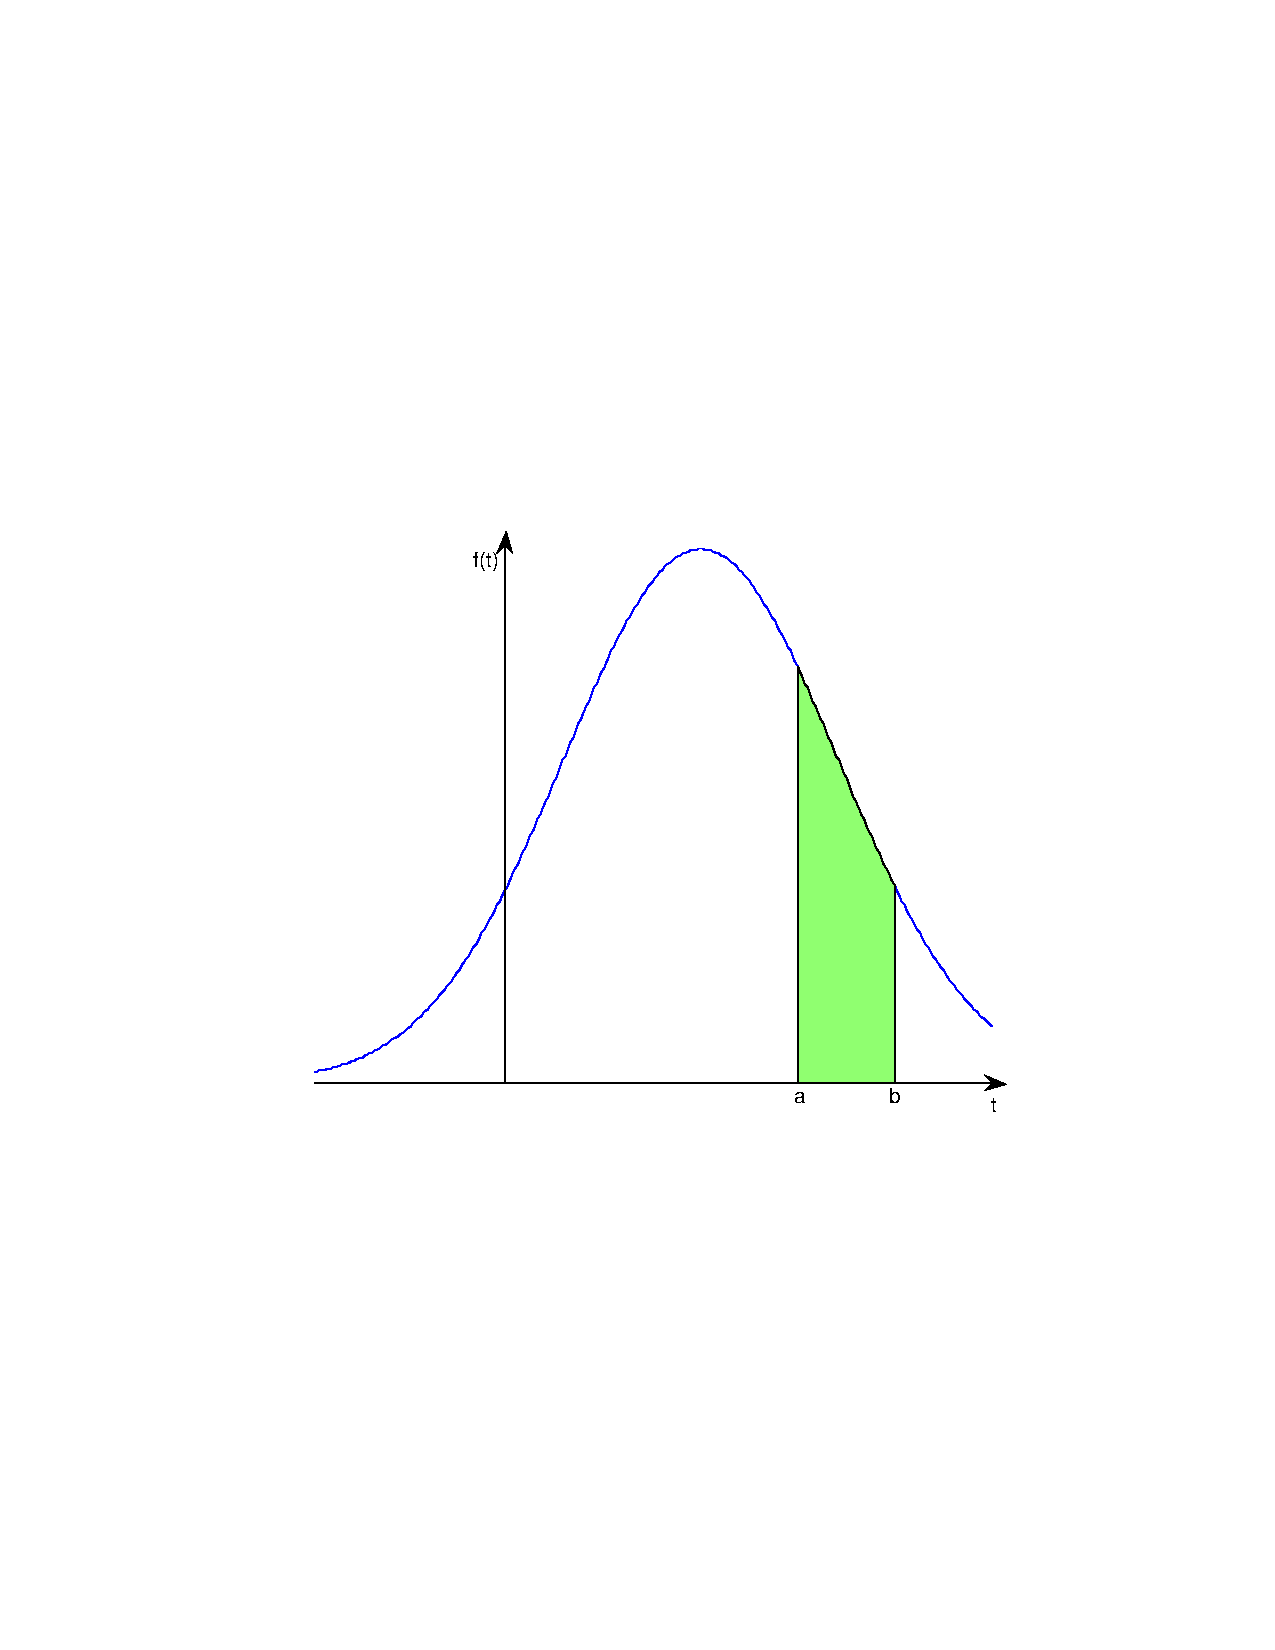
\includegraphics[width=0.5\textwidth]{FIGS/distrib_a_b}
\end{center}
\end{frame}

\begin{frame}\frametitle{Cumulative distribution function}
The cumulative distribution function (c.d.f.) is a function $F(t)$ that characterizes the distribution of $T$, and defined by
\[
F(s)=\IP(T\leq s)=\int_{-\infty}^sf(x)dx
\]
\begin{center}
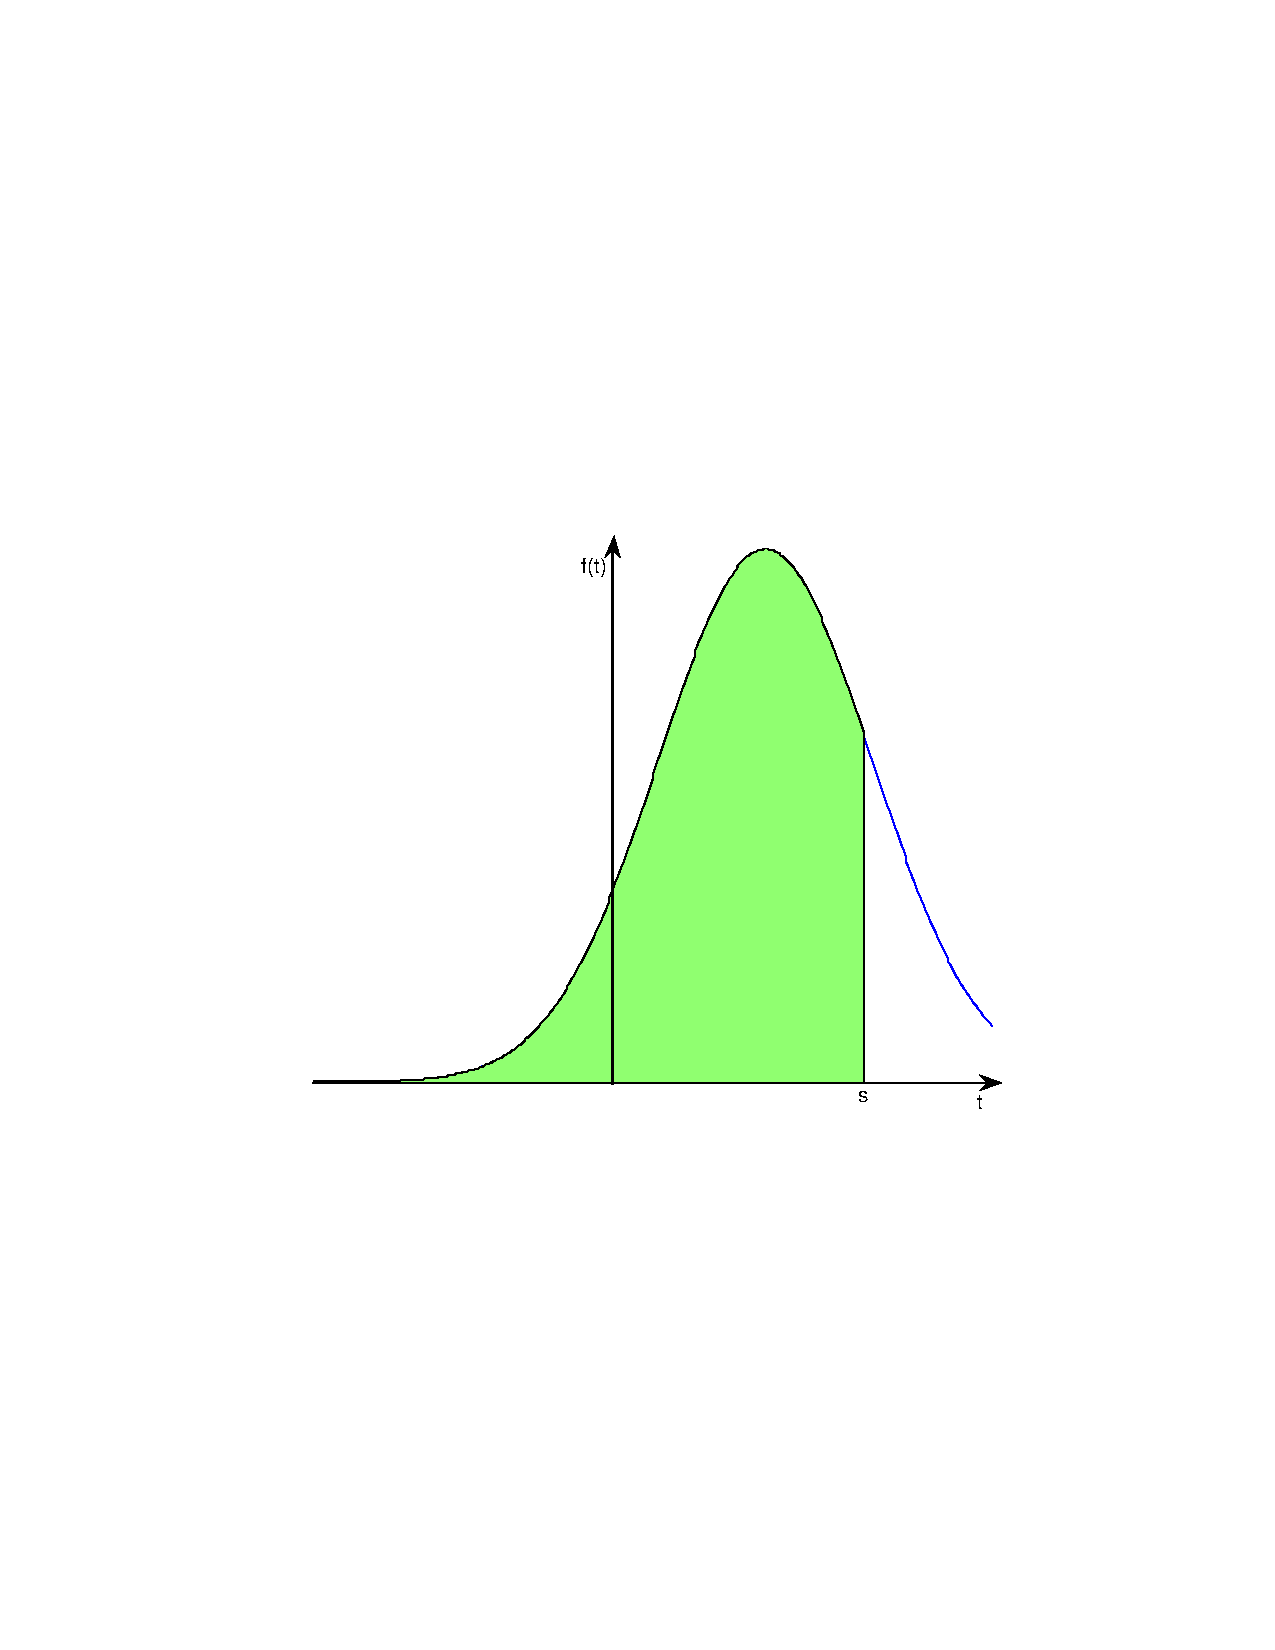
\includegraphics[width=0.5\textwidth]{FIGS/cdf_auc}
\end{center}
\end{frame}

\begin{frame}\frametitle{Survival function}
Another characterization of the distribution of the random variable
$T$ is through the \textbf{survival} (or \textbf{sojourn}) function
\vfill
The survival function of state $S_1$ is given by 
\begin{equation}
  \S(t)=1-F(t)=\IP(T>t)
  \label{eq:survival}
\end{equation}
This gives a description of the \textbf{sojourn time} of a
system in a particular state (the time spent in the state)
\vfill
$\S$ is a nonincreasing function (since $\S=1-F$
with $F$ a c.d.f.), and
$\S(0)=1$ (since $T$ is a nonnegative random variable)
\end{frame}

\begin{frame}
The \textbf{average sojourn time} $\tau$ in state $S_1$ is given by
\[
\tau=E(T)=\int_0^\infty tf(t)dt
\]
Since $\lim_{t\to\infty}t\S(t)=0$, it follows that 
\[
\tau=\int_0^\infty \S(t)dt
\]
\vfill
\textbf{Expected future lifetime}:
\[
\frac{1}{\S(t_0)} \int_0^{\infty} t\,f(t+t_0)\,dt 
\]
\vfill
\begin{eqnarray*}
\S(t)-\S(a)&=&\IP\left\{\textrm{survive during }
 (a,t)\textrm{ having survived until }a\right\} \\
&=& \exp\left(-\int_a^t h(u)du\right)
\end{eqnarray*}
\end{frame}

\begin{frame}\frametitle{Hazard rate}
The \textbf{hazard rate} (or \textbf{failure rate}) is
\begin{align*}
h(t) &= \lim_{\Delta t\to 0}\frac{\S(t)-\S(t+\Delta t)}{\Delta t} \\
& = \lim_{\Delta t\to 0} \frac{\IP{ T<t+\Delta t | T\geq
t}}{\Delta t} \\
&= \frac{f(t)}{\S(t)}
\end{align*}
It gives probability of failure between $t$ and $\Delta t$, given survival to $t$.
\vfill
We have
\[
h(t)=-\frac{d}{dt}\ln\S(t)
\]
\end{frame}

%%%%%%%%%%%%%%%%%%%%%%%%%%%
\begin{frame}{Competing risks}
Suppose now that the system starts in state $A$ at time $t=0$ and that depending on which of the two events $\mathcal{E}_1$ or $\mathcal{E}_2$ takes place first, it switches to state $B_1$ or $B_2$, respectively
\vfill
Consider the random variables $T_A$, \emph{time spent} in state $A$ (or sojourn time in $A$), $T_{AB_1}$, \emph{time before switch to} $B_1$ and $T_{AB_2}$, \emph{time before switch to} $B_2$
\vfill
If we consider state $A$, we cannot observe the variables $T_{AB_1}$ or $T_{AB_2}$. What is observable is the sojourn time in $A$
\[
T^*_A=\min\left( T_{AB_1},T_{AB_2} \right)
\]
(where $^*$ indicates that a quantity is observable)
\end{frame}

\begin{frame}{Taux d'échec par type d'évènement}
We have two (or more) types of events whose individual failure rates have to be accounted for
\begin{align*}
h_j(t) &= \lim_{\Delta t\to 0} \frac{\mathbb{P}( T<t+\Delta t, S=S_j | T\geq t)}{\Delta t} 
\end{align*}
where $\mathbb{P}(T<t+\Delta t, S=S_j | T\geq t)$ is the probability of failure due to cause $S_j$ ($j=1,2$ ici), i.e., $S$ is a discrete r.v. representing the event that is taking place
\end{frame}

\begin{frame}
By the law of total probability, since only one of the event can take place, if there are $n$ risks, then
$$
h(t) = \sum_{i=1}^n h_j(t)
$$
or, identically,
$$
\mathcal{S}(t)
=
\exp\left(
  -\int_0^t \sum\textstyle_{j=1}^n h_j(s)\ ds
\right)
$$
\end{frame}

\begin{frame}
As a consequence, if a process is subject to two competing exponential risks with respective distributions with parameters $\theta_1$ and $\theta_2$, the the mean sojourn time in the initial state before being affected by one of the two risks is
$$
\frac{1}{\theta_1+\theta_2}
$$
\end{frame}


%%%%%%%%%%%%%%%%%%%
%%%%%%%%%%%%%%%%%%%
%%%%%%%%%%%%%%%%%%%
%%%%%%%%%%%%%%%%%%%
\subsection{Two ``extreme'' distributions}

\begin{frame}\frametitle{The exponential distribution}
The random variable $T$ has an \textbf{exponential} distribution if its
probability density function takes the form
\begin{equation}\label{eq:exp_distrib}
f(t)=\begin{cases}0&\textrm{if }t<0,\\
\theta e^{-\theta t}&\textrm{if }t\geq 0,
\end{cases}
\end{equation}
with $\theta>0$. Then the
survival function for state $S_1$ is of the form $\S(t)=e^{-\theta
  t}$, for $t\geq 0$, and the average sojourn time in state $S_1$ is
\[
\tau=\int_0^\infty e^{-\theta t}dt=\frac 1\theta
\]
\end{frame}

\begin{frame}\frametitle{Particularities of the exponential distribution}
The standard deviation of an exponential distribution is also $1/\theta$. When estimating $\theta$, it is impossible to distinguish the mean and the standard deviation
\vfill
The exponential distribution is \textbf{memoryless}: its conditional probability obeys
\[
P(T > s + t\; |\; T > s) = P(T > t),\quad\forall s, t \ge 0
\]

The exponential and geometric distributions are the only memoryless probability distributions
\vfill
The exponential distribution has a constant hazard function
\end{frame}

\begin{frame}\frametitle{The Dirac delta distribution}
If for some constant $\omega>0$,
\[
\S(t)=
\left\{
\begin{array}{ll}
1, & 0\leq t\leq\omega \\
0, & \omega<t
\end{array}
\right.
\]
meaning that $T$ has a Dirac delta distribution
$\delta_\omega(t)$, then the average sojourn time is
\[
\tau=\int_0^\omega dt=\omega
\]
\end{frame}


%%%%%%%%%%%%%%%%%%%
%%%%%%%%%%%%%%%%%%%
%%%%%%%%%%%%%%%%%%%
%%%%%%%%%%%%%%%%%%%
\subsection{A simple cohort model with death} 

\begin{frame}\frametitle{A model for a cohort with one cause of death}
Consider a \textbf{cohort} of individuals born at the same time, e.g., the same year
\vfill
\begin{itemize}
\item At time $t=0$, there are initially $N_0>0$ individuals
\item All causes of death are compounded together 
\item The time until death, for a given individual, is a random variable $T$, with continuous probability density distribution $f(t)$ and survival function $P(t)$
\end{itemize}
\vfill
$N(t)$ the cohort population at time $t\geq 0$
\begin{equation}\label{eq:N_general}
N(t)=N_0P(t)
\end{equation}
\vfill
$N_0P(t)$ proportion of initial population still alive at time $t$
\end{frame}

\begin{frame}\frametitle{Case where $T$ is exponentially distributed}
Suppose that $T$ has an exponential distribution with mean $1/d$ (or parameter $d$), $f(t)=de^{-dt}$. Then the survival function is $P(t)=e^{-dt}$, and \eqref{eq:N_general} takes the form
\begin{equation}\label{eq:N}
N(t)=N_0e^{-dt}
\end{equation}
\vfill
Now note that
\begin{align*}
\frac{d}{dt} N(t) &= -dN_0e^{-dt} \\
&= -dN(t)
\end{align*}
with $N(0)=N_0$.
\vfill
{\red $\Rightarrow$} The ODE $N'=-dN$ makes the assumption that the life expectancy at birth is exponentially distributed
\end{frame}

\begin{frame}
Survival function, $\S(t)=\IP(T>t)$, for an exponential distribution with mean 80 years
\begin{center}
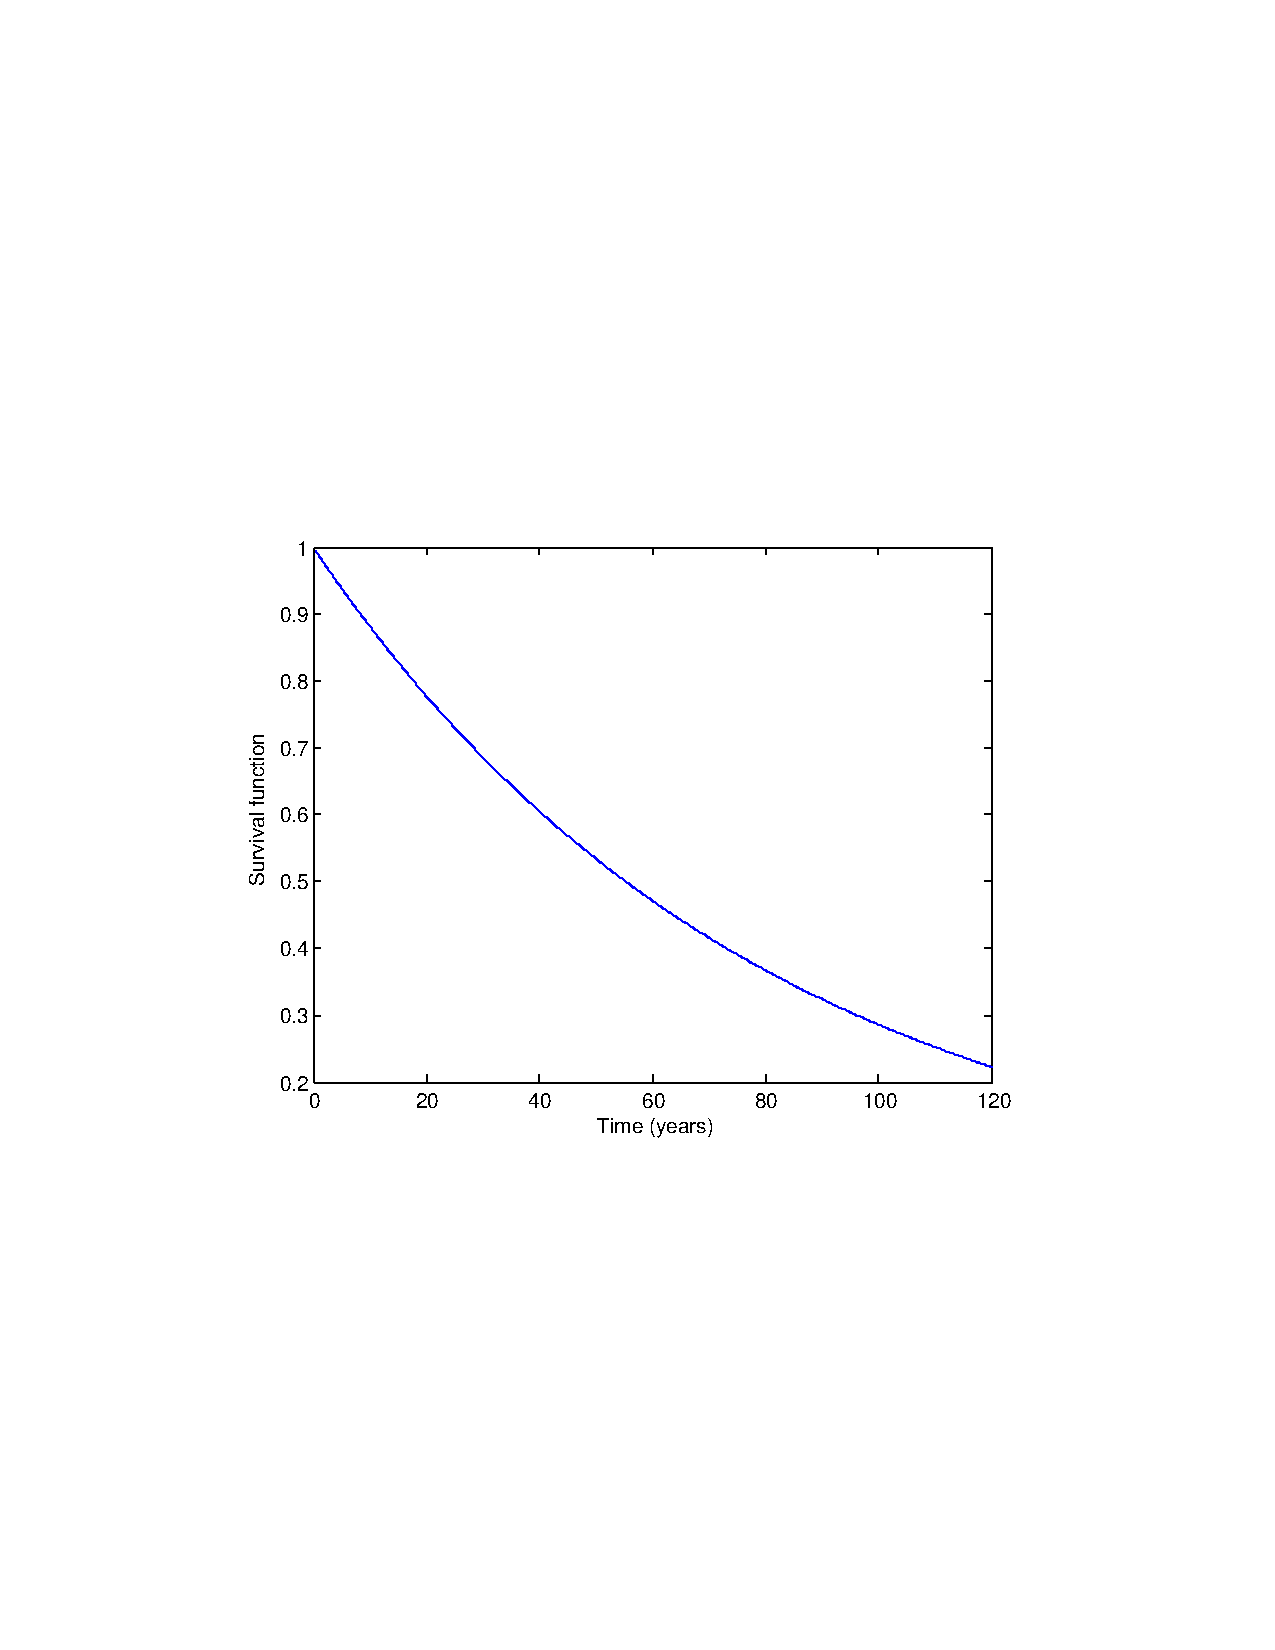
\includegraphics[width=0.7\textwidth]{FIGS/survival_exp_80years}
\end{center}
\end{frame}


\begin{frame}\frametitle{Case where $T$ has a Dirac delta distribution}
Suppose that $T$ has a Dirac delta distribution at $t=\omega$, giving the
survival function 
\[
P(t)=\begin{cases}
1, & 0\leq t\leq\omega,\\
0, & t>\omega.
\end{cases}
\]
Then \eqref{eq:N_general} takes the form
\begin{equation}\label{eq:N2}
N(t)=\begin{cases}
N_0, & 0\leq t\leq\omega,\\
0, & t>\omega.
\end{cases}
\end{equation}
All individuals survive until time $\omega$, then they all die at time $\omega$.
\vfill
Here, we have $N'=0$ everywhere except at $t=\omega$, where it is undefined.
\end{frame}


%%%%%%%%%%%%%%%%%%%
%%%%%%%%%%%%%%%%%%%
%%%%%%%%%%%%%%%%%%%
%%%%%%%%%%%%%%%%%%%
\subsection{Sojourn times in an SIS disease transmission model} 

\begin{frame}\frametitle{An SIS model}
\framesubtitle{Hypotheses}
\begin{itemize}
\item Individuals typically recover from the disease
\item The disease does not confer immunity
\item There is no birth or death (from the disease or natural) \newline\imply\;
Constant total population $N\equiv N(t)=S(t)+I(t)$
\item Infection is of \textbf{standard incidence} type
\end{itemize}
\end{frame}


\begin{frame}\frametitle{Recovery}
\begin{itemize}
\item Traditional models suppose that recovery occurs with rate constant
$\gamma$
\vfill
\item Here, of the individuals that become
infective at time $t_0$, a fraction $P(t-t_0)$ remain infective at
time $t\geq t_0$
\vfill
\item \imply\;
For $t\geq 0$, $P(t)$ is a survival function. As such, it verifies
$P(0)=1$ and $P$ is nonnegative and nonincreasing
\end{itemize}
\end{frame}


\begin{frame}\frametitle{Model for infectious individuals}
Since $N$ is constant, $S(t)=N-I(t)$ and we need only
consider the following equation (where $S$ is used for clarity)
\begin{equation}
I(t) = I_0(t)+ \int_0^t\beta\frac{S(u)I(u)}{N} P(t-u) du
\label{eq:SIS_I} 
\end{equation}
\vfill
\begin{itemize}
\item $I_0(t)$ number of individuals who were infective at time
$t=0$ and still are at time $t$.
\begin{itemize}
\item $I_0(t)$ is nonnegative, nonincreasing, and
such that $\lim_{t\to\infty}I_0(t)=0$.
\end{itemize}
\item $P(t-u)$ proportion of individuals who became infective at time $u$ and who still are at time $t$.
\end{itemize}
\end{frame}


\begin{frame}\frametitle{Expression under the integral}
Integral equation for the number of infective individuals: 
\begin{equation}
I(t) = I_0(t)+ \int_0^t\beta\frac{(N-I(u))I(u)}{N} P(t-u) du
\tag{\ref{eq:SIS_I}} 
\end{equation}
The term
\[
\beta\frac{(N-I(u))I(u)}{N} P(t-u)
\]
\begin{itemize}
\item $\beta (N-I(u))I(u)/N$ is the rate at which new infectives are created, at
time $u$,
\item multiplying by $P(t-u)$ gives the proportion of those who became
infectives at time $u$ and who still are at time $t$.
\end{itemize}
Summing over $[0,t]$ gives the number of infective individuals at time $t$.
\end{frame}


\begin{frame}\frametitle{Case of an exponentially distributed time to recovery}
Suppose $P(t)$ such that sojourn time in the infective
state has exponential distribution with mean $1/\gamma$,
\textbf{i.e.}, $P(t)=e^{-\gamma t}$.
\vfill
Initial condition function $I_0(t)$ takes the form
\[
I_0(t)=I_0(0)e^{-\gamma t},
\]
with $I_0(0)$ the number of infective individuals at time $t=0$. Obtained by considering the cohort of initially infectious individuals, giving a
model such as \eqref{eq:N_general}.
\vfill
Equation (\ref{eq:SIS_I}) becomes
\begin{equation}\label{eq:I_ODE}
I(t)=I_0(0)e^{-\gamma t}+\int_0^t \beta\frac{(N-I(u))I(u)}{N} e^{-\gamma
(t-u)}du.
\end{equation}
\end{frame}

\begin{frame}
Taking the time derivative of \eqref{eq:I_ODE} yields
\begin{align*}
I'(t) &= -\gamma I_0(0)e^{-\gamma t}-\gamma\int_0^t
\beta\frac{(N-I(u))I(u)}{N}e^{-\gamma(t-u)}du \\
&\quad +\beta \frac{(N-I(t))I(t)}{N} \\
&= -\gamma\left(I_0(0)e^{-\gamma t}+
\int_0^t \beta\frac{(N-I(u))I(u)}{N}e^{-\gamma(t-u)}du\right) \\
&\quad +\beta \frac{(N-I(t))I(t)}{N} \\
&= \beta \frac{(N-I(t))I(t)}{N}-\gamma I(t),
\end{align*}
which is the classical logistic type ordinary differential equation
(ODE) for $I$ in an SIS model without vital dynamics (no birth or death).
\end{frame}



\begin{frame}\frametitle{Case of a step function survival function}
Consider case where the time spent infected has survival function 
\[
P(t)=\begin{cases}
1, & 0\leq t\leq\omega,\\
0, & t>\omega.
\end{cases}
\]
i.e., the sojourn time in the infective state is a constant
$\omega>0$.
 
In this case (\ref{eq:SIS_I}) becomes
\begin{equation}\label{eq:I_DDE}
I(t)=I_0(t)+\int_{t-\omega}^t \beta\frac{(N-I(u))I(u)}{N} du.
\end{equation}
Here, it is more difficult to obtain an expression for $I_0(t)$. It is however
assumed that $I_0(t)$ vanishes for $t>\omega$.
\end{frame}

\begin{frame}
When differentiated, \eqref{eq:I_DDE} gives, for $t\geq\omega$,
\[
I'(t)=I_0'(t)+\beta\frac{(N-I(t))I(t)}{N}
-\beta\frac{\left(N-I(t-\omega)\right)I(t-\omega)}{N}.
\]
Since $I_0(t)$ vanishes for $t>\omega$, this gives the delay
differential equation (DDE)
\[
I'(t)=\beta\frac{(N-I(t))I(t)}{N}
-\beta\frac{(N-I(t-\omega))I(t-\omega)}{N}.
\]
\end{frame}




%%%%%%%%%%%%%%%%%%%
%%%%%%%%%%%%%%%%%%%
%%%%%%%%%%%%%%%%%%%
%%%%%%%%%%%%%%%%%%%
\subsection{Conclusion}

\begin{frame}\frametitle{Conclusion}
\begin{itemize}
\item The time of sojourn in classes (compartments) plays an important role in determining the type of model that we deal with
\vfill
\item All ODE models, when they use terms of the form $\kappa X$, make the assumption that the time of sojourn in compartments is exponentially distributed
\vfill
\item At the other end of the spectrum, delay differential with discrete delay make the assumption of a constant sojourn time, equal for all individuals
\vfill
\item Both can be true sometimes.. but reality is more likely somewhere in between
\end{itemize}
\end{frame}

%%%%%%%%%%%%%%%%%%%
%%%%%%%%%%%%%%%%%%%
%%%%%%%%%%%%%%%%%%%
%%%%%%%%%%%%%%%%%%%
\section{Discrete-time Markov chains}

\begin{frame}
A discrete-time Markov chain takes the form
\[
p(n+1)=p(n)P, \quad n=1,2,3,\dots
\]
where $p(n)=(p_1(n),p_{2}(n),\dots , p_r(n))$ is a (row) probability vector and $P=(p_{ij})$ is a $r\times r$ \textbf{transition matrix}
\[
P=
\begin{pmatrix}
p_{11} & p_{12} & \cdots & p_{1r} \\
p_{21} & p_{22} & \cdots & p_{2r} \\
&&& \\
p_{r1} & p_{r2} & \cdots & p_{rr}
\end{pmatrix}
\]
\end{frame}

\begin{frame}{Stochastic matrices}
\begin{definition}
    The nonnegative $r\times r$ matrix $M$ is \textbf{stochastic} if $\sum_{j=1}^ra_{ij}=1$ for all $i=1,2,\dots, r$    
\end{definition}
\vfill
\begin{definition}
Let $M$ be a stochastic matrix $M$. Then all eigenvalues $\lambda$ of $M$ are such that $|\lambda|\leq 1$. Furthermore, $\lambda =1$ is an eigenvalue of $M$
\end{definition}
\vfill
\begin{theorem}
    If $M,N$ are stochastic matrices, then $MN$ is a stochastic matrix
\end{theorem}
\vfill
\begin{theorem}
    If $M$ is a stochastic matrix, then for any $k\in\mathbb{N}$, $M^k$ is a stochastic matrix
\end{theorem}
\end{frame}

\begin{frame}{Asymptotic behavior}
    Let $p(0)$ be the initial distribution (row) vector. Then
\begin{align*}
p(1) &= p(0)P \\
p(2) &= p(1)P\\
&= (p(0)P)P \\
&= p(0)P^2
\end{align*}
Iterating, we get that for any $n$,
$$
p(n)=p(0)P^n
$$
Therefore, 
$$
\lim_{n\rightarrow +\infty}p(n)=\lim_{n\rightarrow +\infty}p(0)P^n=p(0)\lim_{n\rightarrow +\infty}P^n
$$
\end{frame}

%%%%%%%%%%%%%%%%%%%
%%%%%%%%%%%%%%%%%%%
%%%%%%%%%%%%%%%%%%%
%%%%%%%%%%%%%%%%%%%
\subsection{Regular DTMC}

\begin{frame}{Regular Markov chain}
    \begin{definition}
        A \textbf{regular Markov chain} is one in which $P^k$ is positive for some integer $k>0$, i.e., $P^k$ has only positive entries, no zero entries
    \end{definition}    
    \vfill
    \begin{definition}
        A nonnegative matrix $M$ is \textbf{primitive} if, and only if, there is an integer $k>0$ such that $M^k$ is positive
    \end{definition}
    \begin{theorem}
        A Markov chain is regular if, and only if, the transition matrix $P$ is primitive
    \end{theorem}
\end{frame}


\begin{frame}{Important result for regular Markov chains}
    \begin{theorem}
    If $P$ is the transition matrix of a regular Markov chain, then
    \begin{enumerate}
        \item the powers $P^n$ approach a stochastic matrix $W$
        \item each row of $W$ is the same (row) vector $w=(w_1,\ldots,w_r)$
        \item the components of $w$ are positive
    \end{enumerate}
    \end{theorem}
    \vfill
    So if the Markov chain is regular
    $$
    \lim_{n\rightarrow +\infty}p(n)=p(0)\lim_{n\rightarrow +\infty}P^n
    =p(0)W
    $$
\end{frame}


\begin{frame}
    The vector $w$ is the left eigenvector corresponding to the eigenvalue 1 of $P$. (We already know that the (right) eigenvector corresponding to 1 is $\nbOne$.)
\vfill
    Indeed, if $p(n)$ converges, then $p(n+1)=p(n)P$, so $w$ is a fixed point of the system. We thus write
    $$
    wP=w
    $$
    and solve for $w$, which amounts to finding $w$ as the left eigenvector corresponding to the eigenvalue 1
    \vfill
    Alternatively, we can find $w$ as the (right) eigenvector associated to the eigenvalue 1 for the transpose of $P$
    $$
    P^Tw^T=w^T
    $$  
    \vfill
    (normalise if need be)      
\end{frame}


\begin{frame}{Linking matrix and graph theory}
\begin{definition}
    A digraph $\mathcal{G}$ is \textbf{strongly connected} if there is a path between all pairs of vertices
\end{definition}
\vfill
\begin{definition}
    A matrix $M\in\mathcal{M}_n$ is \textbf{irreducible} if there does not exist a matrix $P\in\mathcal{M}_n$ s.t. $P^{-1}AP$ block triangular 
\end{definition}
\vfill
\begin{theorem}
    $A\in\mathcal{M}_n$ irreducible $\iff$ $\mathcal{G}(A)$ strongly connected    
\end{theorem}

\begin{center}
    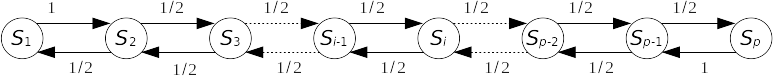
\includegraphics[width=\textwidth]{FIGS/drunk_mans_walk_regular}
    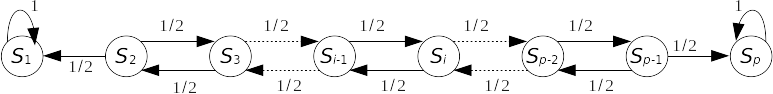
\includegraphics[width=\textwidth]{FIGS/drunk_mans_walk_absorbing}
\end{center}
\end{frame}


%%%%%%%%%%%%%%%%%%%
%%%%%%%%%%%%%%%%%%%
%%%%%%%%%%%%%%%%%%%
%%%%%%%%%%%%%%%%%%%
\subsection{Random walk v1.0 (regular case)}

\begin{frame}{Drunk man's walk 1.0 (regular case)}
    \begin{itemize}
        \item chain of states $S_1,\ldots,S_p$
        \item if in state $S_i$, $i=2,\ldots,p-1$, probability 1/2 of going left (to $S_{i-1}$) and 1/2 of going right (to $S_{i+1}$)
        \item if in state $S_1$, probability 1 of going to $S_2$
        \item if in state $S_p$, probability 1 of going to $S_{p-1}$
    \end{itemize}
\vfill
\begin{center}
    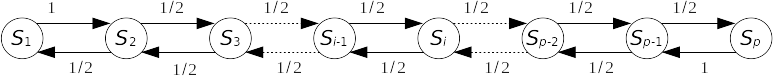
\includegraphics[width=\textwidth]{FIGS/drunk_mans_walk_regular}
\end{center}
\end{frame}


\begin{frame}{Transition matrix for DMW 1.0}
    $$
    P=\begin{pmatrix}
    0 & 1 & 0 & 0 & 0 & \cdots & 0\\
    1/2 & 0 & 1/2 & 0 & & & \\
    0 & 1/2 & 0 & 1/2 & & & \\
    \vdots & & \ddots & \ddots & \ddots & & \vdots \\
    & & & & & & \\
    & & & & 1/2 & 0 & 1/2 \\
    & & & & 0 & 1 & 0
    \end{pmatrix}
    $$
    Clearly a primitive matrix, so a regular Markov chain. We find (easy to do by hand)
    $$
    w^T=\left(\frac{1}{2(p-1)},\frac{1}{p-1},\ldots,\frac{1}{p-1},\frac{1}{2(p-1)}\right)
    $$    
\end{frame}

% <<DTMC-sim-1>>=
% library(markovchain)
% # Total population
% nb_states = 10 # Small so we can see output
% # Parameters
% proba_left = 0.5
% proba_right = 0.5
% proba_stay = 1-(proba_left+proba_right)
% # Make the transition matrix
% T = mat.or.vec(nr = nb_states, nc = nb_states)
% for (row in 2:(nb_states-1)) {
%     T[row,(row-1)] = proba_left
%     T[row,(row+1)] = proba_right
%     T[row, row] = proba_stay
% }
% # First row only has move right
% T[1,2] = 1
% # Last row only has move left
% T[nb_states, (nb_states-1)] = 1
% mcRW <- new("markovchain", 
%             states = sprintf("S_%d", 1:nb_states),
%             transitionMatrix = T,
%             name = "RW_reg")
% @

\begin{frame}[fragile]{Setting up the transition matrix}
\begin{lstlisting}[language=Renhanced]
# Total population
nb_states = 10 # Small so we can see output
# Parameters
proba_left = 0.5
proba_right = 0.5
proba_stay = 1-(proba_left+proba_right)
# Make the transition matrix
T = mat.or.vec(nr = nb_states, nc = nb_states)
for (row in 2:(nb_states-1)) {
    T[row,(row-1)] = proba_left
    T[row,(row+1)] = proba_right
    T[row, row] = proba_stay
}
# First row only has move right
T[1,2] = 1
# Last row only has move left
T[nb_states, (nb_states-1)] = 1
\end{lstlisting}
\end{frame}

\begin{frame}[fragile]{Analysis using \code{markovchain} library}
\begin{lstlisting}[language=Renhanced]
library(markovchain)
mcRW <- new("markovchain", 
            states = sprintf("S_%d", 1:nb_states),
            transitionMatrix = T,
            name = "RW_reg")
\end{lstlisting}
\vfill
\begin{lstlisting}
> summary(mcRW)
RW_reg  Markov chain that is composed by: 
Closed classes: 
S_1 S_2 S_3 S_4 S_5 S_6 S_7 S_8 S_9 S_10 
Recurrent classes: 
{S_1,S_2,S_3,S_4,S_5,S_6,S_7,S_8,S_9,S_10}
Transient classes: 
NONE 
The Markov chain is irreducible 
The absorbing states are: NONE
\end{lstlisting}
\end{frame}


\begin{frame}[fragile]
\begin{lstlisting}
> steadyStates(mcRW)
            S_1       S_2       S_3       S_4       S_5       S_6       S_7       S_8       S_9
[1,] 0.05555556 0.1111111 0.1111111 0.1111111 0.1111111 0.1111111 0.1111111 0.1111111 0.1111111
           S_10
[1,] 0.05555556
\end{lstlisting}
\vfill
Jives with 
$$
w^T=\left(\frac{1}{2(p-1)},\frac{1}{p-1},\ldots,\frac{1}{p-1},\frac{1}{2(p-1)}\right)
$$
we had computed
\end{frame}

\begin{frame}[fragile]
\code{meanRecurrenceTime}: outputs a named vector with the expected time to first return to a state when the chain starts there. States present in the vector are only the recurrent ones. If the matrix is ergodic (i.e. irreducible), then all states are present in the output and order is the same as states order for the Markov chain
\begin{lstlisting}[language=Renhanced]
> meanRecurrenceTime(mcRW)
 S_1  S_2  S_3  S_4  S_5  S_6  S_7  S_8  S_9 S_10 
  18    9    9    9    9    9    9    9    9   18 
\end{lstlisting}
\vfill
\code{period}: returns a integer number corresponding to the periodicity of the Markov chain (if it is irreducible)
\begin{lstlisting}[language=Renhanced]
> period(mcRW)
[1] 2
\end{lstlisting}
(period of state $x\in\mathcal{S}$ is $\gcd\{n\in\mathbb{N}_+: T^n(x,x)>0\}$)
\end{frame}

\begin{frame}[fragile]
\code{meanFirstPassageTime}: Given an irreducible (ergodic) \code{markovchain} object, this function calculates the expected number of steps to reach other states

\begin{lstlisting}[language=Renhanced]
> meanFirstPassageTime(mcRW)
     S_1 S_2 S_3 S_4 S_5 S_6 S_7 S_8 S_9 S_10
S_1    0   1   4   9  16  25  36  49  64   81
S_2   17   0   3   8  15  24  35  48  63   80
S_3   32  15   0   5  12  21  32  45  60   77
S_4   45  28  13   0   7  16  27  40  55   72
S_5   56  39  24  11   0   9  20  33  48   65
S_6   65  48  33  20   9   0  11  24  39   56
S_7   72  55  40  27  16   7   0  13  28   45
S_8   77  60  45  32  21  12   5   0  15   32
S_9   80  63  48  35  24  15   8   3   0   17
S_10  81  64  49  36  25  16   9   4   1    0
\end{lstlisting}
\end{frame}
%%%%%%%%%%%%%%%%%%%
%%%%%%%%%%%%%%%%%%%
%%%%%%%%%%%%%%%%%%%
%%%%%%%%%%%%%%%%%%%
\subsection{Absorbing DTMC}

\begin{frame}{Absorbing states, absorbing chains}
    \begin{definition}
        A state $S_i$ in a Markov chain is \textbf{absorbing} if whenever it occurs on the $n^{th}$ generation of the experiment, it then occurs on every subsequent step. In other words, $S_i$ is absorbing if $p_{ii}=1$ and $p_{ij}=0$ for $i\neq j$
    \end{definition}
    \begin{definition}
        A \textbf{Markov chain is absorbing} if it has at least one absorbing state, and if from every state it is possible to go to an absorbing state
    \end{definition}
    \begin{definition}
        In an absorbing Markov chain, a state that is not absorbing is called \textbf{transient}
    \end{definition}
\end{frame}

\begin{frame}{Some questions on absorbing chains}
    Suppose we have a chain like the following
    \begin{center}
        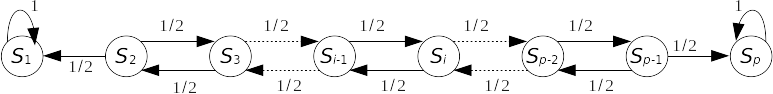
\includegraphics[width=\textwidth]{FIGS/drunk_mans_walk_absorbing}
    \end{center}
    \begin{enumerate}
        \item Does the process eventually reach an absorbing state?
        \item Average number of times spent in a transient state, if starting in a transient state?
        \item Average number of steps before entering an absorbing state?
        \item Probability of being absorbed by a given absorbing state, when there are more than one, when starting in a given transient state?
    \end{enumerate}
\end{frame}



\begin{frame}{Reaching an absorbing state}
    Answer to question 1:
    \begin{theorem}
        In an absorbing Markov chain, the probability of reaching an absorbing state is 1
    \end{theorem}
\end{frame}

\begin{frame}{Standard form of the transition matrix}
    For an absorbing chain with $k$ absorbing states and $r-k$ transient states, the transition matrix can be written as
    $$
    P=\begin{pmatrix}
    \mathbb{I}_k & \mathbf{0} \\
    R & Q
    \end{pmatrix}
    $$
    
    \begin{center}
        \begin{tabular}{c|c|c|}
            & Absorbing states & Transient states \\
            \hline
            \textbf{Absorbing states} & $\mathbb{I}_k$ & $\mathbf{0}$ \\
            \textbf{Transient states} & $R$ & $Q$ 
        \end{tabular}
    \end{center}
    \vfill
    $\mathbb{I}_k$ the $k\times k$ identity, $\mathbf{0}\in\mathbb{R}^{k\times(r-k)}$, $R\in\mathbb{R}^{(r-k)\times k}$, $Q\in\mathbb{R}^{(r-k)\times(r-k)}$
\end{frame}


\begin{frame}
    The matrix $\mathbb{I}_{r-k}-Q$ is invertible. Let
\begin{itemize}
    \item $N=(\mathbb{I}_{r-k}-Q)^{-1}$ be the \textbf{fundamental matrix} of the Markov chain
    \item $T_i$ be the sum of the entries on row $i$ of $N$
    \item $B=NR$
\end{itemize}
\vfill
Answers to our remaining questions:

\begin{enumerate}
    \setcounter{enumi}{1}
    \item $N_{ij}$ is the average number of times the process is in the $j$th transient state if it starts in the $i$th transient state
    \item $T_i$ is the average number of steps before the process enters an absorbing state if it starts in the $i$th transient state
    \item $B_{ij}$ is the probability of eventually entering the $j$th absorbing state if the process starts in the $i$th transient state
\end{enumerate}
\vfill
See for instance book of \href{https://www.amazon.com/Finite-Markov-Chains-Laurie-Kemeny/dp/B000KYES0O}{Kemeny and Snell}
\end{frame}


\begin{frame}{Drunk man's walk 2.0 (absorbing case)}
    \begin{itemize}
        \item chain of states $S_1,\ldots,S_p$
        \item if in state $S_i$, $i=2,\ldots,p-1$, probability 1/2 of going left (to $S_{i-1}$) and 1/2 of going right (to $S_{i+1}$)
        \item if in state $S_1$, probability 1 of going to $S_1$
        \item if in state $S_p$, probability 1 of going to $S_p$
    \end{itemize}
    \vfill
\begin{center}
    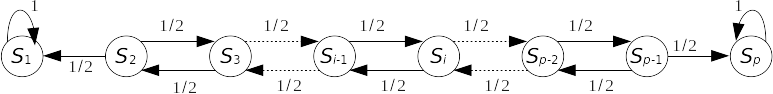
\includegraphics[width=\textwidth]{FIGS/drunk_mans_walk_absorbing}
\end{center}
\end{frame}


\begin{frame}{Transition matrix for DMW 2.0}
    $$
    P=\begin{pmatrix}
    1 & 0 & 0 & 0 & 0 & \cdots & 0\\
    1/2 & 0 & 1/2 & 0 & & & \\
    0 & 1/2 & 0 & 1/2 & & & \\
    \vdots & & \ddots & \ddots & \ddots & & \vdots \\
    & & & & & & \\
    & & & & 1/2 & 0 & 1/2 \\
    & & & & 0 & 0 & 1
    \end{pmatrix}
    $$    
\end{frame}


\begin{frame}{Put $P$ in standard form}
    Absorbing states are $S_1$ and $S_p$, write them first, then write other states

    \begin{center}
        \begin{tabular}{c|cccccccc}
            & $S_1$ & $S_p$ & $S_2$ & $S_3$ & $S_4$ & $\cdots$ & $S_{p-2}$ & $S_{p-1}$ \\
            \hline 
            $S_1$ & 1 & 0 & 0 & 0 & 0 & $\cdots$ & 0 & 0 \\
            $S_p$ & 0 & 1 & 0 & 0 & 0 & $\cdots$ & 0 & 0 \\
            $S_2$ & 1/2 & 0 & 0 & 1/2 & 0 & $\cdots$ & 0 & 0 \\
            $S_3$ & 0 & 0 & 1/2 & 0 & 1/2 & $\cdots$ & 0 & 0 \\
            $\vdots$ &  &  &  &  & & & & \\
            $S_{p-2}$ & 0 & 0 & 0 & 0 & 0 & $\cdots$ & 0 & 1/2 \\
            $S_{p-1}$ & 0 & 1/2 & 0 & 0 & 0 & $\cdots$ & 1/2 & 0                 
        \end{tabular}
    \end{center}
\end{frame}

\begin{frame}
    So we find
    $$
    P=\begin{pmatrix}
    \mathbb{I}_2 & \mathbf{0} \\
    R & Q
    \end{pmatrix}
    $$
    where $\mathbf{0}$ a $2\times(p-2)$-matrix, $R$ a $(p-2)\times 2$ matrix and $Q$ a $(p-2)\times (p-2)$ matrix
\end{frame}


\begin{frame}
    $$
    R=
    \begin{pmatrix}
    1/2 & 0 \\
    0 & 0 \\
    \vdots & \vdots \\
    0 & 0 \\
    0 & 1/2   
    \end{pmatrix}
    $$
    and
    $$
    Q=
    \begin{pmatrix}
    0 & 1/2 & 0 & \\
    1/2 & 0 & 1/2 & \\
    0 & 1/2 & 0 & \\
    && \ddots & \ddots & \ddots \\
    &&&& \\
    0 &&& 1/2 & 0 & 1/2 \\
    0 &&&&1/2 & 0
    \end{pmatrix}
    $$
\end{frame}


\begin{frame}
    $$
    \mathbb{I}_{p-2}-Q=
    \begin{pmatrix}
    1 & -1/2 & 0 & \\
    -1/2 & 1 & -1/2 & \\
    0 & -1/2 & 1 & \\
    && \ddots & \ddots & \ddots \\
    &&&& \\
    0 &&& -1/2 & 1 & -1/2 \\
    0 &&&& -1/2 & 1
    \end{pmatrix}
    $$
    \vfill
    This is a \textbf{symmetric tridiagonal Toeplitz} matrix 
    \vfill
    (symmetric: obvious; tridiagonal: there are three diagonal bands; Toeplitz: each diagonal band is constant)
    \vfill
    Could invert it explicitly, let us not bother
\end{frame}

% <<absorbing-DTMC>>=
% # Total population
% nb_states = 10 # Small so we see output
% # Parameters
% proba_left = 0.5
% proba_right = 0.5
% proba_stay = 1-(proba_left+proba_right)
% # Make the transition matrix
% T = mat.or.vec(nr = nb_states, nc = nb_states)
% for (row in 2:(nb_states-1)) {
%     T[row,(row-1)] = proba_left
%     T[row,(row+1)] = proba_right
%     T[row, row] = proba_stay
% }
% # First and last rows only have stay
% T[1,1] = 1
% T[nb_states, nb_states] = 1    
% library(markovchain)
% mcRW <- new("markovchain", 
%             states = sprintf("S_%d", 1:nb_states),
%             transitionMatrix = T,
%             name = "RW_abs")
% @

\begin{frame}[fragile]{Setting up the transition matrix}
\begin{lstlisting}[language=Renhanced]
# Total population
nb_states = 10 # Small so we see output
# Parameters
proba_left = 0.5
proba_right = 0.5
proba_stay = 1-(proba_left+proba_right)
# Make the transition matrix
T = mat.or.vec(nr = nb_states, nc = nb_states)
for (row in 2:(nb_states-1)) {
    T[row,(row-1)] = proba_left
    T[row,(row+1)] = proba_right
    T[row, row] = proba_stay
}
# First and last rows only have stay
T[1,1] = 1
T[nb_states, nb_states] = 1    
\end{lstlisting}
\end{frame}

\begin{frame}[fragile]{Analysis using \code{markovchain} library}
\begin{lstlisting}
library(markovchain)
mcRW <- new("markovchain", 
            states = sprintf("S_%d", 1:nb_states),
            transitionMatrix = T,
            name = "RW_abs")
\end{lstlisting}
\vfill
\begin{lstlisting}[language=Renhanced]
> summary(mcRW)
RW_abs  Markov chain that is composed by: 
Closed classes: 
S_1 
S_10 
Recurrent classes: 
{S_1},{S_10}
Transient classes: 
{S_2,S_3,S_4,S_5,S_6,S_7,S_8,S_9}
The Markov chain is not irreducible 
The absorbing states are: S_1 S_10
\end{lstlisting}
\end{frame}

\begin{frame}[fragile]
\begin{lstlisting}
> canonicForm(mcRW)
RW_abs 
    A  10 - dimensional discrete Markov Chain defined by the following states: 
    S_1, S_10, S_2, S_3, S_4, S_5, S_6, S_7, S_8, S_9 
    The transition matrix  (by rows)  is defined as follows: 
        S_1 S_10 S_2 S_3 S_4 S_5 S_6 S_7 S_8 S_9
S_1  1.0  0.0 0.0 0.0 0.0 0.0 0.0 0.0 0.0 0.0
S_10 0.0  1.0 0.0 0.0 0.0 0.0 0.0 0.0 0.0 0.0
S_2  0.5  0.0 0.0 0.5 0.0 0.0 0.0 0.0 0.0 0.0
S_3  0.0  0.0 0.5 0.0 0.5 0.0 0.0 0.0 0.0 0.0
S_4  0.0  0.0 0.0 0.5 0.0 0.5 0.0 0.0 0.0 0.0
S_5  0.0  0.0 0.0 0.0 0.5 0.0 0.5 0.0 0.0 0.0
S_6  0.0  0.0 0.0 0.0 0.0 0.5 0.0 0.5 0.0 0.0
S_7  0.0  0.0 0.0 0.0 0.0 0.0 0.5 0.0 0.5 0.0
S_8  0.0  0.0 0.0 0.0 0.0 0.0 0.0 0.5 0.0 0.5
S_9  0.0  0.5 0.0 0.0 0.0 0.0 0.0 0.0 0.5 0.0
\end{lstlisting}
\end{frame}



\begin{frame}[fragile]
\begin{lstlisting}
> meanAbsorptionTime(mcRW)
S_2 S_3 S_4 S_5 S_6 S_7 S_8 S_9 
    8  14  18  20  20  18  14   8 
> absorptionProbabilities(mcRW)
            S_1      S_10
S_2 0.8888889 0.1111111
S_3 0.7777778 0.2222222
S_4 0.6666667 0.3333333
S_5 0.5555556 0.4444444
S_6 0.4444444 0.5555556
S_7 0.3333333 0.6666667
S_8 0.2222222 0.7777778
S_9 0.1111111 0.8888889
\end{lstlisting}
\end{frame}


\begin{frame}[fragile]
\code{hittingProbabilities}: given a \code{markovchain} object, this function calculates the probability of ever arriving from state i to j

\begin{lstlisting}
> hittingProbabilities(mcRW)
            S_1    S_2       S_3       S_4   S_5   S_6       S_7       S_8    S_9      S_10
S_1  1.0000000 0.0000 0.0000000 0.0000000 0.000 0.000 0.0000000 0.0000000 0.0000 0.0000000
S_2  0.8888889 0.4375 0.5000000 0.3333333 0.250 0.200 0.1666667 0.1428571 0.1250 0.1111111
S_3  0.7777778 0.8750 0.6785714 0.6666667 0.500 0.400 0.3333333 0.2857143 0.2500 0.2222222
S_4  0.6666667 0.7500 0.8571429 0.7500000 0.750 0.600 0.5000000 0.4285714 0.3750 0.3333333
S_5  0.5555556 0.6250 0.7142857 0.8333333 0.775 0.800 0.6666667 0.5714286 0.5000 0.4444444
S_6  0.4444444 0.5000 0.5714286 0.6666667 0.800 0.775 0.8333333 0.7142857 0.6250 0.5555556
S_7  0.3333333 0.3750 0.4285714 0.5000000 0.600 0.750 0.7500000 0.8571429 0.7500 0.6666667
S_8  0.2222222 0.2500 0.2857143 0.3333333 0.400 0.500 0.6666667 0.6785714 0.8750 0.7777778
S_9  0.1111111 0.1250 0.1428571 0.1666667 0.200 0.250 0.3333333 0.5000000 0.4375 0.8888889
S_10 0.0000000 0.0000 0.0000000 0.0000000 0.000 0.000 0.0000000 0.0000000 0.0000 1.0000000
\end{lstlisting}
\end{frame}

\begin{frame}{DTMC SIS system}
    Since $S=P^\star-I$, consider only the infected. To simulate as DTMC, consider a random walk on $I$ ($\simeq$ Gambler's ruin problem)
    \vfill
    Denote $\lambda_I = \beta (P^\star-I)I\Delta t$, $\mu_I = \gamma I\Delta t$ and $\sigma_I=1-(\lambda_I+\mu_I)\Delta t$
    \vfill
    \begin{center}
        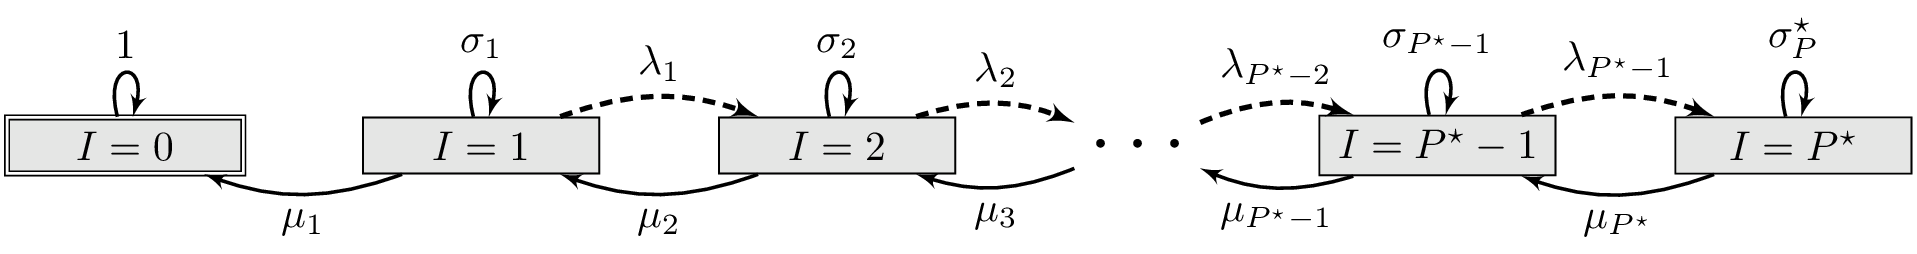
\includegraphics[width=\textwidth]{FIGS/figure_SIS_random_walk.png}
    \end{center}
\end{frame}


% \begin{frame}{Transition matrix}
% \[
% A = 
% \begin{pmatrix}
% 1 & 0 &&&&&&&&&
%     \mu_1 & \sigma_1 & \lambda_1 & 0 &&&&&&& \\
%     0 & \mu_2 & \sigma_2 & \lambda_2 & 0 &&&&&& \\
%     &&&&&&&&&& \\
%     &&&&& \ddots &&&&& \\
%     &&&&&&&&&& \\
%     &&&&&& 0 & \mu_{P^\star-1} & \mu_{P^\star-1} & \lambda_{P^\star-1} & 0 \\
%     &&&&&&&& 0 & \mu_{P^\star} & \sigma_{P^\star}
% \end{pmatrix}
% \]
% \end{frame}


\begin{frame}[fragile]
    To make things easy to see: \code{Pop=5}
\begin{lstlisting}
# Make the transition matrix
T = mat.or.vec(nr = (Pop+1), nc = (Pop+1))
for (row in 2:Pop) {
    I = row-1
    mv_right = gamma*I*Delta_t # Recoveries
    mv_left = beta*I*(Pop-I)*Delta_t # Infections
    T[row,(row-1)] = mv_right
    T[row,(row+1)] = mv_left
}
# Last row only has move left
T[(Pop+1),Pop] = gamma*(Pop)*Delta_t
# Check that we don't have too large values
if (max(rowSums(T))>1) {
    T = T/max(rowSums(T))
}
diag(T) = 1-rowSums(T)    
\end{lstlisting}
\end{frame}


\begin{frame}[fragile]{Analysis using \code{markovchain} library}
\begin{lstlisting}
library(markovchain)
mcSIS <- new("markovchain", 
                states = sprintf("I_%d", 0:Pop),
                transitionMatrix = T,
                name = "SIS")    
\end{lstlisting}
\vfill
\begin{lstlisting}
> summary(mcSIS)
SIS  Markov chain that is composed by: 
Closed classes: 
I_0 
Recurrent classes: 
{I_0}
Transient classes: 
{I_1,I_2,I_3,I_4,I_5}
The Markov chain is not irreducible 
The absorbing states are: I_0    
\end{lstlisting}
\end{frame}


\begin{frame}[fragile]
\begin{lstlisting}
> canonicForm(mcSIS)
SIS 
    A  6 - dimensional discrete Markov Chain defined by the following states: 
    I_0, I_1, I_2, I_3, I_4, I_5 
    The transition matrix  (by rows)  is defined as follows: 
            I_0       I_1       I_2       I_3       I_4       I_5
I_0 1.0000000 0.0000000 0.0000000 0.0000000 0.0000000 0.0000000
I_1 0.1666667 0.5000000 0.3333333 0.0000000 0.0000000 0.0000000
I_2 0.0000000 0.3333333 0.1666667 0.5000000 0.0000000 0.0000000
I_3 0.0000000 0.0000000 0.5000000 0.0000000 0.5000000 0.0000000
I_4 0.0000000 0.0000000 0.0000000 0.6666667 0.0000000 0.3333333
I_5 0.0000000 0.0000000 0.0000000 0.0000000 0.8333333 0.1666667    
\end{lstlisting}
\end{frame}


\begin{frame}[fragile]
\begin{lstlisting}
# The vector of steady states. Here, all mass should be in I_0
> steadyStates(mcSIS)
        I_0 I_1 I_2 I_3 I_4 I_5
[1,]   1   0   0   0   0   0    
\end{lstlisting}
\vfill
\begin{lstlisting}
> hittingProbabilities(mcSIS)
    I_0       I_1       I_2       I_3       I_4       I_5
I_0   1 0.0000000 0.0000000 0.0000000 0.0000000 0.0000000
I_1   1 0.8333333 0.6666667 0.5454545 0.4615385 0.3529412
I_2   1 1.0000000 0.8888889 0.8181818 0.6923077 0.5294118
I_3   1 1.0000000 1.0000000 0.9090909 0.8461538 0.6470588
I_4   1 1.0000000 1.0000000 1.0000000 0.8974359 0.7647059
I_5   1 1.0000000 1.0000000 1.0000000 1.0000000 0.8039216
\end{lstlisting}
Read by row: if the process starts in $I_i$ (row $i-1$), probability that state $I_j$ (column $j-1$) is visited
\end{frame}

\begin{frame}[fragile]
\begin{lstlisting}
> meanAbsorptionTime(mcSIS)
    I_1   I_2   I_3   I_4   I_5 
  24.30 33.45 37.55 39.65 40.85 
> absorptionProbabilities(mcSIS)
  I_0
  I_1   1
  I_2   1
  I_3   1
  I_4   1
  I_5   1      
\end{lstlisting}
\end{frame}

%%%%%%%%%%%%%%%%%%%
%%%%%%%%%%%%%%%%%%%
%%%%%%%%%%%%%%%%%%%
%%%%%%%%%%%%%%%%%%%
\section{Continuous time Markov chains}

\begin{frame}{Continuous-time Markov chains}
    CTMC similar to DTMC except in way they handle time between events (transitions)
\vfill
    DTMC: transitions occur each $\Delta t$
   \vfill 
    CTMC: $\Delta t\to 0$ and transition times follow an exponential distribution parametrised by the state of the system
    \vfill
    CTMC are roughly equivalent to ODE    
\end{frame}


\subsection{ODE $\leftrightarrow$ CTMC}

\begin{frame}{Converting your compartmental ODE model to CTMC}
    Easy as $\pi$ :)
\vfill
\begin{itemize}
    \item Compartmental ODE model focuses on flows into and out of compartments
    \item ODE model has as many equations as there are compartments
    \item Compartmental CTMC model focuses on transitions
    \item CTMC model has as many transitions as there are arrows between (or into or out of) compartments
\end{itemize}
\end{frame}


\begin{frame}{ODE to CTMC : focus on different components}
    \begin{center}
        \begin{tikzpicture}[auto,
            scale=1.2, every node/.style={transform shape},
            cloud/.style={minimum width={width("N-1")+2pt},
            draw, ellipse,fill=red!20}]
            \node[cloud, fill=green!90, double=red] (S) at (0,0) {$S$};
            \node[cloud, draw=none, fill=white] (h4) at (2,0) {};
            \node[cloud, fill=red!90, double=red] (I) at (4,0) {$I$};
            \node[cloud, fill=green!90] (S2) at (6,0) {$S$};
            \node[cloud, fill=red!90] (I2) at (8,0) {$I$};
            %% Flows (ODE)
            \path [line, bend left, very thick, dashed] (S) to node [midway, above] (TextNode) {$-\beta SI$} (h4);
            \path [line, bend left, very thick] (h4) to node [midway, below] (TextNode) {$+\gamma I$} (S);
            \path [line, bend left, very thick] (h4) to node [midway, above] (TextNode) {$+\beta SI$} (I);
            \path [line, bend left, very thick, dashed] (I) to node [midway, below] (TextNode) {$-\gamma I$} (h4);
            %% Flows (CTMC)
            \path [line, bend left, very thick, red] (S2) to node [midway, above, black] (TextNode) {$\beta SI$} (I2);
            \path [line, bend left, very thick, red] (I2) to node [midway, below] (TextNode) {$\gamma I$} (S2);
            %%
            \draw[very thick, dotted] (5,-2) -- (5,2);
            %%
            \node[style=rectangle] at (2,2) {ODE};
            \node[style=rectangle] at (7,2) {CTMC};
            %%
            \node[style=rectangle] (fODE) at (2,-2) {focus};
            \path [line, dotted,red] (fODE) to  (S.south);
            \path [line, dotted,red] (fODE) to  (I.south);
            \node[style=rectangle] (fCTMC) at (6,-2) {focus};
            \path [line, dotted,red] (fCTMC) to (6.75,0.3);
            \path [line, dotted,red] (fCTMC) to  (6.75,-0.475);
        \end{tikzpicture}        
    \end{center}
\end{frame}


\begin{frame}{SIS without demography}
    \begin{center}
        \begin{tabular}{cp{3cm}cc}
            Transition & Effect & Weight & Probability \\
            $S\to S-1$, $I\to I+1$ & new infection & $\beta SI$ & $\dfrac{\beta SI}{\beta SI+\gamma I}$ \\
            $S\to S+1$, $I\to I-1$ & recovery of an infectious & $\gamma I$ & $\dfrac{\gamma I}{\beta SI+\gamma I}$
        \end{tabular}
    \end{center}
    \vfill
    States are $S,I$
\end{frame}


\begin{frame}{SIS with demography}
    \begin{center}
        \begin{tabular}{p{3cm}p{3cm}cc}
            Transition & Effect & Weight & Probability \\
            $S\to S+1$ & birth of a susceptible & $b$ & $\frac{b}{b+d(S+I)+\beta SI+\gamma I}$ \\
            $S\to S-1$ & death of a susceptible & $dS$ & $\frac{dS}{b+d(S+I)+\beta SI+\gamma I}$ \\
            $S\to S-1$, $I\to I+1$ & new infection & $\beta SI$ & $\frac{\beta SI}{b+d(S+I)+\beta SI+\gamma I}$ \\
            $I\to I-1$ & death of an infectious & $dI$ & $\frac{dI}{b+d(S+I)+\beta SI+\gamma I}$ \\
            $S\to S+1$, $I\to I-1$ & recovery of an infectious & $\gamma I$ & $\frac{\gamma I}{b+d(S+I)+\beta SI+\gamma I}$ 
        \end{tabular}
    \end{center}
\vfill
States are $S,I$
\end{frame}


\begin{frame}[fragile]{Kermack \& McKendrick model}
    \begin{center}
        \begin{tabular}{cp{3cm}cc}
            Transition & Effect & Weight & Probability \\
            $S\to S-1$, $I\to I+1$ & new infection & $\beta SI$ & $\dfrac{\beta SI}{\beta SI+\gamma I}$ \\
            $I\to I-1$, $R\to R+1$ & recovery of an infectious & $\gamma I$ & $\dfrac{\gamma I}{\beta SI+\gamma I}$ 
        \end{tabular}
    \end{center}
    \vfill
    States are $S,I,R$
\end{frame}


\subsection{Simulating CTMC (in theory)}

\begin{frame}{Gillespie's algorithm}
    \begin{itemize}
        \item A.k.a. the stochastic simulation algorithm (SSA)
        \item Derived in 1976 by Daniel Gillespie
        \item Generates possible solutions for CTMC
        \item Extremely simple, so worth learning how to implement; there are however packages that you can use (see later)
    \end{itemize}
\end{frame}


\begin{frame}{Gillespie's algorithm}
Suppose system has state $\mathbf{x}(t)$ with initial condition $\mathbf{x}(t_0)=\mathbf{x}_0$ and \emph{propensity functions} $a_i$ of elementary reactions
\vfill
set $t\leftarrow t_0$ and $\mathbf{x}(t)\leftarrow \mathbf{x}_0$\\
while {$t\leq t_f$}\\
- $\xi_t\leftarrow \sum_j a_j(\mathbf{x}(t))$\\
- Draw $\tau_t$ from $T\thicksim \mathcal{E}(\xi_t)$\\
- Draw $\zeta_t$ from $\mathcal{U}([0,1])$\\
- Find $r$, smallest integer s.t. $\sum_{k=1}^j a_k(\mathbf{x}(t))> \zeta_t\sum_j a_j(\mathbf{x}(t))=\zeta_t\xi_t$\\
- Effect the next reaction (the one indexed $r$)\\
- $t\leftarrow t+\tau_t$\\    
\end{frame}


\begin{frame}{Drawing at random from an exponential distribution}
    If you do not have an exponential distribution random number generator.. We want $\tau_t$ from $T\thicksim\mathcal{E}(\xi_t)$, i.e., $T$ has probability density function
    $$
    f(x,\xi_t)=
    \xi_te^{-\xi_t x}\mathbf{1}_{x\geq 0}
    $$
    Use cumulative distribution function $F(x,\xi_t)=\int_{-\infty}^x f(s,\xi_t)\,ds$
    $$
    F(x,\xi_t)=
    (1-e^{-\xi_t x})\mathbf{1}_{x\geq 0}
    $$
    which has values in $[0,1]$. So draw $\zeta$ from $\mathcal{U}([0,1])$ and solve $F(x,\xi_t)=\zeta$ for $x$
    \begin{align*}
    F(x,\xi_t)=\zeta & \Leftrightarrow 1-e^{-\xi_tx}=\zeta \\
    &\Leftrightarrow e^{-\xi_tx} = 1-\zeta \\
    &\Leftrightarrow \xi_tx = -\ln(1-\zeta) \\
    &\Leftrightarrow \boxed{x = \frac{-\ln(1-\zeta)}{\xi_t}}
    \end{align*}
\end{frame}


\begin{frame}{Gillespie's algorithm (SIS model with only I eq.)}
set $t\leftarrow t_0$ and $I(t)\leftarrow I(t_0)$\\
while {$t\leq t_f$}\\
- $\xi_t\leftarrow \beta (P^\star-i)i+\gamma i$\\
- Draw $\tau_t$ from $T\thicksim \mathcal{E}(\xi_t)$\\
- $v\leftarrow\left[\beta (P^\star-i)i,\xi_t\right]/\xi_t$\\
- Draw $\zeta_t$ from $\mathcal{U}([0,1])$\\
- Find $pos$ such that $v_{pos-1}\leq\zeta_t\leq v_{pos}$\\
- switch {$pos$}\\
\qquad - 1: New infection, $I(t+\tau_t)=I(t)+1$ \\
\qquad - 2: End of infectious period, $I(t+\tau_t)=I(t)-1$ \\
- $t\leftarrow t+\tau_t$
\end{frame}


\begin{frame}{Sometimes Gillespie goes bad}
    \begin{itemize}
        \item Recall that the inter-event time is exponentially distributed
        \item Critical step of the Gillespie algorithm:
        \begin{itemize}
            \item $\xi_t\leftarrow$ weight of all possible events (\emph{propensity})
            \item Draw $\tau_t$ from $T\thicksim \mathcal{E}(\xi_t)$
        \end{itemize}
        \item So the inter-event time $\tau_t\to 0$ if $\xi_t$ becomes very large for some $t$
        \item This can cause the simulation to grind to a halt
    \end{itemize}
\end{frame}


\begin{frame}{Example: a birth and death process}
    \begin{itemize}
        \item Individuals born at \emph{per capita} rate $b$
        \item Individuals die at \emph{per capita} rate $d$
        \item Let's implement this using classic Gillespie
    \end{itemize}
    \vfill
(See \href{https://raw.githubusercontent.com/julien-arino/3MC-course-epidemiological-modelling/main/CODE/simulate_birth_death_CTMC.R}{\code{simulate\_birth\_death\_CTMC.R}} on course GitHub repo)
\end{frame}


\begin{frame}{Gillespie's algorithm (birth-death model)}
set $t\leftarrow t_0$ and $N(t)\leftarrow N(t_0)$\\
while {$t\leq t_f$}\\
- $\xi_t\leftarrow (b+d)N(t)$\\
- Draw $\tau_t$ from $T\thicksim \mathcal{E}(\xi_t)$\\
- $v\leftarrow\left[bN(t),\xi_t\right]/\xi_t$\\
- Draw $\zeta_t$ from $\mathcal{U}([0,1])$\\
- Find $pos$ such that $v_{pos-1}\leq\zeta_t\leq v_{pos}$\\
- switch {$pos$}\\
\qquad - 1: Birth, $N(t+\tau_t)=N(t)+1$ \\
\qquad - 2: Death, $N(t+\tau_t)=N(t)-1$ \\
- $t\leftarrow t+\tau_t$    
\end{frame}

% <<>>=
% b = 0.01   # Birth rate
% d = 0.01   # Death rate
% t_0 = 0    # Initial time
% N_0 = 100  # Initial population
% 
% # Vectors to store time and state. Initialise with initial condition.
% t = t_0
% N = N_0
% 
% t_f = 1000  # Final time
% 
% # We'll track the current time and state (could also just check last entry in t
% # and N, but will take more operations)
% t_curr = t_0
% N_curr = N_0
% while (t_curr<=t_f) {
%     xi_t = (b+d)*N_curr
%     # The exponential number generator does not like a rate of 0 (when the 
%     # population crashes), so we check if we need to quit
%     if (N_curr == 0) {
%         break
%     }
%     tau_t = rexp(1, rate = xi_t)
%     t_curr = t_curr+tau_t
%     v = c(b*N_curr, xi_t)/xi_t
%     zeta_t = runif(n = 1)
%     pos = findInterval(zeta_t, v)+1
%     switch(pos,
%             { 
%                 N_curr = N_curr+1 # Birth
%             },
%             {
%                 N_curr = N_curr-1 # Death
%             })
%     N = c(N, N_curr)
%     t = c(t, t_curr)
% }
% @

\begin{frame}[fragile]
\begin{lstlisting}[language=Renhanced]
b = 0.01   # Birth rate
d = 0.01   # Death rate
t_0 = 0    # Initial time
N_0 = 100  # Initial population

# Vectors to store time and state. Initialise with initial condition.
t = t_0
N = N_0

t_f = 1000  # Final time

# We'll track the current time and state (could also just check last entry in t
# and N, but will take more operations)
t_curr = t_0
N_curr = N_0
\end{lstlisting}
\end{frame}

\begin{frame}[fragile]
\begin{lstlisting}[language=Renhanced]
while (t_curr<=t_f) {
    xi_t = (b+d)*N_curr
    # The exponential number generator does not like a rate of 0 (when the 
    # population crashes), so we check if we need to quit
    if (N_curr == 0) {
        break
    }
    tau_t = rexp(1, rate = xi_t)
    t_curr = t_curr+tau_t
    v = c(b*N_curr, xi_t)/xi_t
    zeta_t = runif(n = 1)
    pos = findInterval(zeta_t, v)+1
    switch(pos,
            { 
                N_curr = N_curr+1 # Birth
            },
            {
                N_curr = N_curr-1 # Death
            })
    N = c(N, N_curr)
    t = c(t, t_curr)
}
\end{lstlisting}
\end{frame}

\maxFrameImage{FIGS/CTMC_birth_death_sol_b=0_01_d=0_01}
\maxFrameImage{FIGS/CTMC_birth_death_sol_b=0_01_d=0_02}
\maxFrameImage{FIGS/CTMC_birth_death_sol_b=0_03_d=0_01}


\begin{frame}[fragile]{Last one did not go well}
    \begin{itemize}
        \item Wanted 1000 time units (days?)
        \item Interrupted at $t=344.4432$ because I lost patience
        \newline (Penultimate slide: sim stopped because the population went extinct, I did not stop it!)
        \item At stop time
        \begin{itemize}
            \item $N = 103,646$
            \item $|N| = 208,217$ (and $|t|$ as well, of course!)
            \item time was moving slowly
        \end{itemize}
    \end{itemize}
    \vfill
    \begin{lstlisting}
> tail(diff(t))
[1] 1.282040e-05 5.386999e-04 5.468540e-04 1.779985e-04 6.737294e-05 2.618084e-04
    \end{lstlisting}
\end{frame}


\maxFrameImage{FIGS/CTMC_birth_death_ie_vs_t_b=0_03_d=0_01}

\subsection{Simulating CTMC (in practice)}

\begin{frame}{Tau-leaping (and packages) to the rescue!}
    \begin{itemize}
        \item \emph{Approximation} method (compared to classic Gillespie, which is exact)
        \item Roughly: consider "groups" of events instead of individual events
        \item Good news: \code{GillespieSSA2} and \code{adaptivetau}, two standard packages for SSA in \code{R}, implement tau leaping
    \end{itemize}
\end{frame}

% <<sim-gillespie2-first,echo=FALSE>>=
% library(GillespieSSA2)
% Pop <- 1000
% I_0 <- 2
% IC <- c(S = (Pop-I_0), I = I_0)
% params <- c(gamma = gamma, beta = beta)
% reactions <- list(
%   reaction("beta*S*I", c(S=-1,I=+1), "new_infection"),
%   reaction("gamma*I", c(S=+1,I=-1), "recovery")
% )
% set.seed(NULL)
% sol <- ssa(
%   initial_state = IC,
%   reactions = reactions,
%   params = params,
%   method = ssa_exact(),
%   final_time = t_f,
% )
% plot(sol$time, sol$state[,"I"], type = "l",
%      xlab = "Time (days)", ylab = "Number infectious")    
% @

\begin{frame}[fragile]{Simulating a CTMC}
\begin{lstlisting}[language=Renhanced]
library(GillespieSSA2)
IC <- c(S = (Pop-I_0), I = I_0)
params <- c(gamma = gamma, beta = beta)
reactions <- list(
    reaction("beta*S*I", c(S=-1,I=+1), "new_infection"),
    reaction("gamma*I", c(S=+1,I=-1), "recovery")
)
set.seed(NULL)
sol <- ssa(
    initial_state = IC,
    reactions = reactions,
    params = params,
    method = ssa_exact(),
    final_time = t_f,
)
plot(sol$time, sol$state[,"I"], type = "l",
        xlab = "Time (days)", ylab = "Number infectious")    
\end{lstlisting}
\end{frame}

\maxFrameImage{FIGS/one_CTMC_sim}

\subsection{Parallelising your code in \code{R}}

\begin{frame}{Parallelisation}
    To see multiple realisations: good idea to parallelise, then interpolate results. Write a function, e.g.,  \code{run\_one\_sim} that .. runs one simulation
    \vfill
    On the GitHub repo for the course, see
    \begin{itemize}
        \item \href{https://raw.githubusercontent.com/julien-arino/3MC-mathematical-modelling-in-biology/main/CODE/Julien/SIS_CTMC_parallel.R}{\code{SIS\_CTMC\_parallel.R}}
        \item \href{https://raw.githubusercontent.com/julien-arino/3MC-mathematical-modelling-in-biology/main/CODE/Julien/SIS_CTMC_parallel_multiple_R0.R}{\code{SIS\_CTMC\_parallel\_multiple\_R0.R}}
    \end{itemize}
\end{frame}

% <<parallel-CTMC>>=
% library(parallel)
% run_one_sim = function(params) {
%     IC <- c(S = (params$Pop-params$I_0), I = params$I_0)
%     params_local <- c(gamma = params$gamma, beta = params$beta)
%     reactions <- list(
%         # propensity function effects name for reaction
%         reaction("beta*S*I", c(S=-1,I=+1), "new_infection"),
%         reaction("gamma*I", c(S=+1,I=-1), "recovery")
%     )
%     set.seed(NULL)
%     sol <- ssa(
%     initial_state = IC,
%     reactions = reactions,
%     params = params_local,
%     method = ssa_exact(),
%     final_time = params$t_f,
%     log_firings = TRUE    # This way we keep track of events
%     )
%     # Interpolate result (just I will do)
%     wanted_t = seq(from = 0, to = params$t_f, by = 0.01)
%     sol$interp_I = approx(x = sol$time, y = sol$state[,"I"], xout = wanted_t)
%     names(sol$interp_I) = c("time", "I")
%     # Return result
%     return(sol)
% }
% nb_cores <- detectCores()
% if (nb_cores > 124) {
%   nb_cores = 124
% }
% cl <- makeCluster(nb_cores)
% clusterEvalQ(cl,{
%   library(GillespieSSA2)
% })
% clusterExport(cl,
%               c("params",
%                 "run_one_sim"),
%               envir = .GlobalEnv)
% SIMS = parLapply(cl = cl, 
%                  X = 1:params$number_sims, 
%                  fun =  function(x) run_one_sim(params))
% stopCluster(cl)
% @

\begin{frame}[fragile]
\begin{lstlisting}[language=Renhanced]
run_one_sim = function(params) {
    IC <- c(S = (params$Pop-params$I_0), I = params$I_0)
    params_local <- c(gamma = params$gamma, beta = params$beta)
    reactions <- list(
        # propensity function effects name for reaction
        reaction("beta*S*I", c(S=-1,I=+1), "new_infection"),
        reaction("gamma*I", c(S=+1,I=-1), "recovery")
    )
    set.seed(NULL)
    sol <- ssa(
    initial_state = IC,
    reactions = reactions,
    params = params_local,
    method = ssa_exact(),
    final_time = params$t_f,
    log_firings = TRUE    # This way we keep track of events
    )
\end{lstlisting}    
\end{frame}

\begin{frame}[fragile]
    \begin{lstlisting}[language=Renhanced]
    # Interpolate result (just I will do)
    wanted_t = seq(from = 0, to = params$t_f, by = 0.01)
    sol$interp_I = approx(x = sol$time, y = sol$state[,"I"], xout = wanted_t)
    names(sol$interp_I) = c("time", "I")
    # Return result
    return(sol)
}
\end{lstlisting}    
\end{frame}


\begin{frame}[fragile]
\begin{lstlisting}[language=Renhanced]
nb_cores <- detectCores()
if (nb_cores > 124) {
    nb_cores = 124
}
cl <- makeCluster(nb_cores)
clusterEvalQ(cl,{
    library(GillespieSSA2)
})
clusterExport(cl,
                c("params",
                "run_one_sim"),
                envir = .GlobalEnv)
SIMS = parLapply(cl = cl, 
                    X = 1:params$number_sims, 
                    fun =  function(x) run_one_sim(params))
stopCluster(cl)
\end{lstlisting}
\end{frame}



% \begin{frame}[fragile]{Parallelisation}    
%then..
% \begin{lstlisting}[language=Renhanced]
% no_cores <- detectCores()-1
% cl <- makeCluster(no_cores)
% clusterEvalQ(cl,{
%     library(GillespieSSA2)
% })
% clusterExport(cl,
%                 c("params",
%                 "run_one_sim"),
%                 envir = .GlobalEnv)
% SIMS = parLapply(cl = cl, 
%                     X = 1:params$number_sims, 
%                     fun =  function(x) run_one_sim(params))
% stopCluster(cl)
% \end{lstlisting}
% See \code{simulate_CTMC_parallel.R} on \href{https://github.com/julien-arino/UK-APASI}{Github}
% \end{frame}

\maxFrameImage{FIGS/many_CTMC_sims_with_means}

\begin{frame}[fragile]{Benefit of parallelisation}    
    Run the parallel code for 100 sims between `tictoc::tic()` and `tictoc::toc()`, giving `66.958 sec elapsed`, then the sequential version
\begin{lstlisting}
tictoc::tic()
SIMS = lapply(X = 1:params$number_sims, 
                FUN =  function(x) run_one_sim(params))
tictoc::toc()
\end{lstlisting}
    which gives `318.141 sec elapsed` on a 6C/12T Intel(R) Core(TM) i9-8950HK CPU @ 2.90GHz (4.75$\times$ faster) or `12.067 sec elapsed` versus `258.985 sec elapsed` on a 32C/64T AMD Ryzen Threadripper 3970X 32-Core Processor (21.46$\times$ faster !)
\end{frame}



\end{document}
